\documentclass[article,A4,12pt]{llncs}
\usepackage[T1]{fontenc}
\usepackage{amsmath}
\usepackage{amssymb}
\usepackage{amsfonts}
\usepackage{mathrsfs, bm}

\usepackage{graphicx}
\usepackage{tabularx}
\usepackage{subfig}
\usepackage{epsf,times}
\usepackage{color}
\usepackage{wrapfig}
\usepackage{cases}
\usepackage{multicol}

\usepackage[T1]{fontenc}
%\newcommand{\tmname}[1]{\textsc{#1}}
%\newcommand{\tmop}[1]{\ensuremath{\operatorname{#1}}}
%\newcommand{\tmsamp}[1]{\textsf{#1}}
%\newcommand{\tmtextsc}[1]{{\scshape{#1}}}
%\newcommand{\tmtextsl}[1]{{\slshape{#1}}}
%\newcommand{\tmtexttt}[1]{{\ttfamily{#1}}}

\leftmargin=0.0cm
\oddsidemargin=0.5cm
\evensidemargin=0.5cm
\topmargin=0cm
\textwidth=16.0cm
%\textheight=21.5cm
\textheight=20.0cm
\pagestyle{plain}
\setlength{\columnsep}{20pt}

\def\m{\mathbf{m}}
\def\H{\mathbf{H}}
\def\E{\mathbf{E}}
\newcommand{\vepsi}{{\varepsilon}}
\def\hnorm#1#2{\vert\,#1\,\vert_{#2}}
\newcommand{\R}{{\mathbb R}}
\newcommand{\Sph}{{\mathbb S}}
\def\x{\mathbf{x}}
\def\hvec{\overline{\mathbf{h}}}
\def\evec{\overline{\mathbf{e}}}

\newcommand{ \etal}{\mbox{\emph{et al. }}}

\newcommand\vect[1]{\mbf{#1}}
\newcommand{\mbf}[1]{\mbox{\boldmath$#1$}} 
\newcommand{\RC}[1]{#1 $\times$ #1 $\times$ #1}
\def\um{$\mu$m}
\def\C{$^{\circ}\mathrm{C}$}

\newcommand{\Rmnum}[1]{\expandafter\@slowromancap\romannumeral #1@}

% DEFINITION OF CUSTOM FONT SIZE
\newcommand{\customfontA}{\fontsize{50}{55}\selectfont}
\newcommand{\customfontB}{\fontsize{14.4}{20}\selectfont}
\newcommand{\customfontC}{\fontsize{30}{35}\selectfont}

\DeclareMathAlphabet{\mathpzc}{OT1}{pzc}{m}{it}

\def\clovek#1{\noindent\bgroup\vbox{\noindent#1}\egroup\vskip1em}

% TO INPUT BACKGROUND IMAGE
\usepackage{eso-pic}
\newcommand\BackgroundPic{
\put(0,0){
\parbox[b][\paperheight]{\paperwidth}{
\vfill
\centering
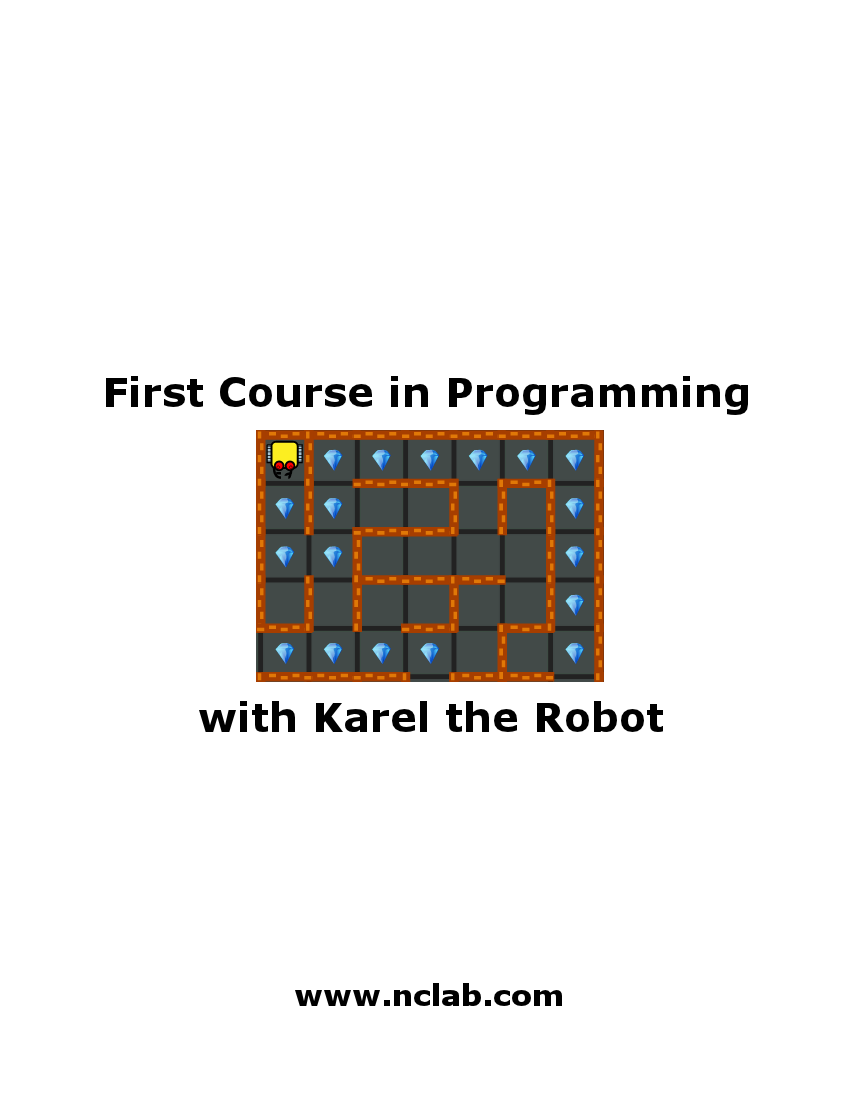
\includegraphics[width=\paperwidth,height=\paperheight]{img/karel-frontpage.png}
%\includegraphics[width=\paperwidth,height=\paperheight]{img/background.jpg}
\vfill
}}}

\begin{document}

% INPUTTING BACKGROUND IMAGE
\AddToShipoutPicture{\BackgroundPic}
\vbox{}
\pagestyle{empty}
\newpage
\textwidth=15.5cm
\ClearShipoutPicture
\newpage

%%%%%%%%%%%%%%%%%%%%%%%%%%%%%%%%%%%%%%%%%%%%%%%%%%%%%%%%%%%%%%%%%%%%%%%%%

\section*{}
\small
\subsection*{About NCLab}
Networked Computing Laboratory (NCLab) is a popular Internet-based framework for 
programming, mathematics, computer modeling, 
and scientific computing. It serves students, instructors, researchers, and the general 
public. NCLab can be used free of charge for personal non-commercial purposes such as 
private hobby or self-education, as well as for individual non-funded academic research.
All other use is subject to {\bf purchasing a license} for a symbolic fee. The fees are as low as 
\$1 per user per month for educational use, and they are used to support the development 
and operational expenses. NCLab is a product of FEMhub Inc. The name "NCLab" is 
registered with the U.S. Patent and Trademark Office (USPTO) under Trademark No. 85420518.

\subsection*{Terms of Use and Pricing}
More details on purchasing a license and using NCLab are provided in the online documents 
{\bf Pricing} and {\bf Terms of Use} that are accessible from NCLab's home page 
{\tt http://nclab.com}.

\subsection*{Contact Information}
General inquiries: {\tt info@femhub.com}\\
Sales: {\tt sales@femhub.com}\\
NCLab support: {\tt support@nclab.com}\\
Agros \& Hermes support: {\tt support@femhub.com}\\
Web page: {\tt http://femhub.com}\\
{Physical address}\\
FEMhub Inc.\\
5490 Twin Creeks Dr.\\
Reno, NV 89523

\subsection*{About This Publication}
This publication can be copied and distributed without any restrictions
as long as reference to NCLab and FEMhub Inc. is preserved.

\subsection*{NCLab's Karel vs. the Original Version}
This publication features {\em Karel the Robot}, a programming language 
designed by Richard E. Pattis. Compared to its original version that was
strongly influenced by Pascal, the NCLab version is closer to Python.
There are some other differences as well that make Karel in NCLab easier to use 
for kids -- Karel collects gems instead of beepers, he has a home in the 
maze, and he uses commands that are much easier for kids to understand
and type. For example, {\tt pickbeeper} was replaced with {\tt get}, 
{\tt front-is-clear} was replaced with {\tt wall}, etc. Even the Python 
colons following every command are omitted because using the SHIFT key 
was causing difficulties to some 5 years old programmers. 
Otherwise we have not changed Pattis' original ideas and all functionality 
covered in Pattis' book is available in the Basic Version of the Programming
module free of charge. 

\normalsize

\newpage
%{\ }
\setcounter{tocdepth}{2}
\tableofcontents
%\pagestyle{plain}

\newpage

\pagestyle{plain}
\setcounter{page}{1}

%%%%%%%%%%%%%%%%%%%%%%%%%%%%%%%%%%%%%%%%%%%%%%%%%%%%%%%%%%%%%%%%%%%%%%%%%

\section{Introduction}

In this introductory course you will learn principles of computer programming with the 
help of an interactive graphical application {\em Karel the Robot} in NCLab. 

\subsection{Brief history}

Karel the Robot is a famous educational programming language that was introduced by Richard E. 
Pattis in his book "Karel The Robot: A Gentle Introduction to the Art of Programming" in 1981. 
Pattis first used the language in his courses at Stanford University, and now it is used at 
countless schools in the world to introduce students to algorithmic design and computer programming. 
The language is named after Karel \v{C}apek, a Czech writer who invented the word "robot" in his 1921 
science fiction play R.U.R. (Rossum's Universal Robots).

\subsection{Who is Karel?}

Karel is a little robot that lives in a maze. The maze contains gems that Karel enjoys to collect. 
He only knows a handful of simple commands such as {\tt go} one step forward, {\tt get} a gem, 
{\tt turn} left, and {\tt put} a gem on the ground. It has built-in sensors that allow him to 
check if a {\tt wall} is in his way, if a {\tt gem} is within his reach, if he is facing {\tt north}, 
if he is at {\tt home}, and if his bag is {\tt empty}. With your help, Karel will learn new things 
that will make it a better Robot, and on the way you will become a Programmer without even noticing! 

\subsection{What is the one reason why I should learn Karel?}

You will learn to {\em design good algorithms} -- an ability that makes
a great programmer and that is completely language-independent. In other 
words, you can learn the same with a technically complicated conventional 
programming language, battling technical problems most of the time,
or you can learn it with Karel the easy way.
Despite its simple form, Karel is not a toy language. It contains all elements 
of a modern procedural programming language. The complexity of algorithms 
covered in this course ranges from {\em very simple} to {\em very tough}.

\subsection{How does Karel differ from conventional programming languages?}

The biggest difference between Karel and all conventional 
programming languages is that it {\em does not involve any mathematics}.
Believe it or not -- Karel does not know numbers. Thanks 
to this, {\em programming concepts} stand out clearly. 
After you finish this tutorial, you will find that suddenly it is very simple 
to learn other languages such as Python or C++, because they are in fact 
very similar to Karel. You will be only learning language-specific details, 
because the most important thing -- algorithmic thinking -- you will already 
know.
 
\section{Getting Started}

In order to make the most of this tutorial, we invite the 
reader to create an account in NCLab and log in. More instructions 
on how to do this are given at the beginning of the introductory 
tutorial "Meet Your New Graphing Calculator" that is available in 
PDF via a link on NCLab home page {\tt http://nclab.com}.\\

\noindent
After logging in, you will see a desktop with several icons on it,
as shown in Fig. \ref{fig:desktop}. 

\begin{figure}[!ht]
\begin{center}
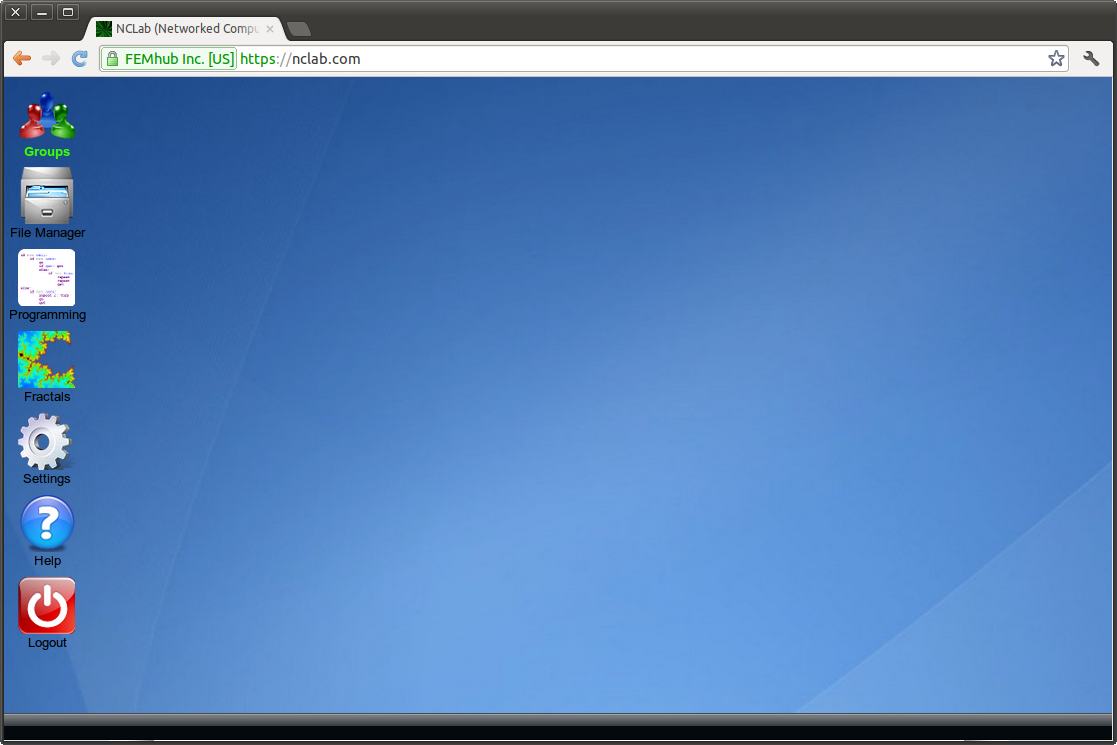
\includegraphics[width=\textwidth]{img/desktop.png}
\end{center}
%\vspace{-2mm}
\caption{NCLab desktop after login}
\label{fig:desktop}
\end{figure}

\subsection{Launching Karel via the Programming icon}

Karel can be launched in several ways. The simplest one is to click on the icon 
"Programming" and select "Karel" in the menu. This will launch the application 
and load a randomly selected maze, as shown in Fig. \ref{fig:init}.

\begin{figure}[!ht]
\begin{center}
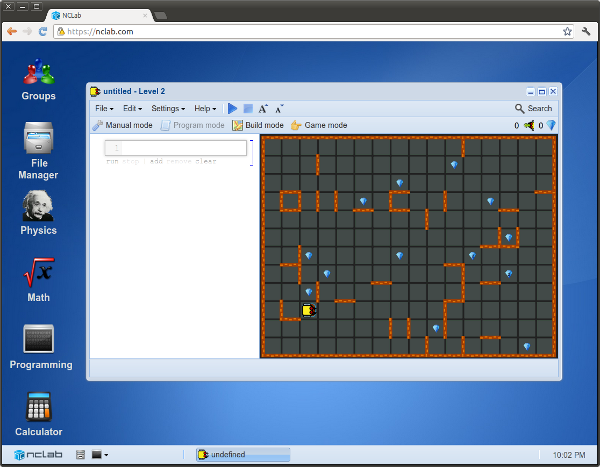
\includegraphics[width=\textwidth]{img/init.png}
\end{center}
%\vspace{-2mm}
\caption{Launching Karel via the Programming icon}
\label{fig:init}
\end{figure}
\noindent
Karel will be launched in {\em Programming mode} which is the most-frequently 
used mode. You can easily switch to the {\em Manual mode}, {\em Builder},
and {\em Game mode} in the menu. Game mode is available in Full Version only. 
These modes will be discussed in more detail later.

\subsection{Cloning Karel projects} \label{cloning}

All programs and games that we will work with in this course are
available for you to clone (download) into your account. To do this, 
click on the File Manager icon. In the File Manager's menu go to 
"Project" and click on "Clone". This will launch a new window with public
projects as shown in Fig. \ref{fig:cloning}. There are many public
projects to choose from so their loading may take a while. 

\newpage

\begin{figure}[!ht]
\begin{center}
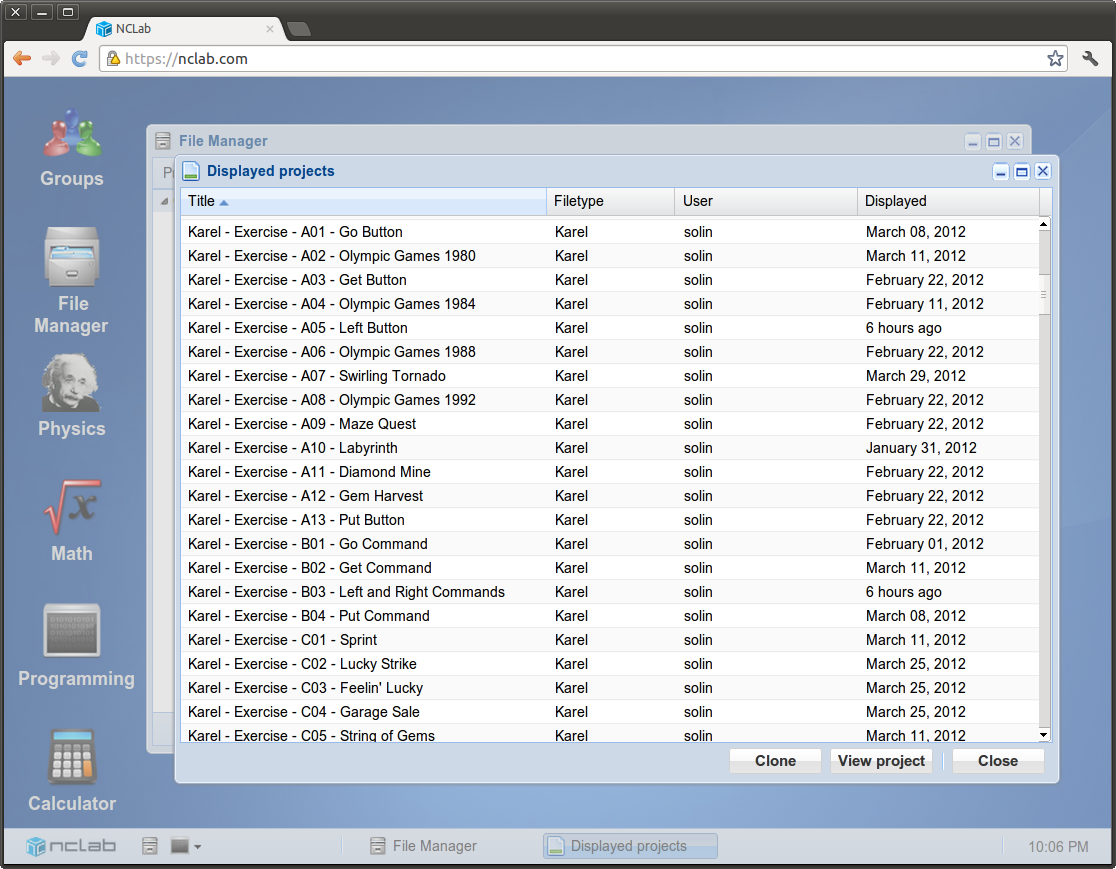
\includegraphics[width=\textwidth]{img/cloning.png}
\end{center}
%\vspace{-2mm}
\caption{Window with public projects is accessible through File Manager's "Project" menu}
\label{fig:cloning}
\end{figure}
\noindent
All projects that have "Karel" in the Engine column are of interest to you. 
Projects whose names start with "Tutorial - A...", "Tutorial - B..." and 
"Tutorial - C..." are of particular interest. This is done via clicking on the project 
name in the window, and pressing the button "Clone". When you are done, close the 
window. 

In the File Manager's right-hand side panel, you will see the list of all 
projects that you cloned. Click on any of them to launch it. You are free to 
use the cloned projects as they are, or modify them in any way you like. Your modifications 
will not affect the public version of the project. And, you can 
always synchronize your version of the project with the public version, via 
a right-click on the project in the File Manager and selecting "Synchronize".
Beware though -- this will erase any changes that you made to the project.

\subsection{Basic and Full Versions}

If you are using the Programming Module in Basic Version, some restrictions apply: The 
number of projects that you can have at any time is limited to 10, and you cannot have
private projects. Specifically in Karel, the Basic Version does not have the Game mode 
enabled. Besides this, the Basic Version of Karel is fully functional without any other 
limitations. 

If you are logged with an institution code, your Programming module is
probably in Full Version and you should not experience any limitations. If you are 
not logged in with an institution code, you can use the desktop icon "Upgrade" 
to upgrade the Programming module to Full Version.

\subsection{Karel modes}

Karel can operate in four modes:
\begin{itemize}
\item {\em Manual mode:} The robot can be controlled using the mouse and four buttons Go, Get, Turn, and Put. Watch out and do not crash!
\item {\em Program mode:} The robot can be controlled using programs. For simplicity, the Program mode is split into Levels:
\begin{itemize}
\item Level 1 is a transition layer from Manual mode to programming. Programs are written using the commands {\tt go}, {\tt get}, {\tt turn} and {\tt put} that are fully equivalent to pressing the buttons Go, Get, Turn and Put in Manual mode, respectively.
\item Level 2 is where the actual programming begins. On top of the commands from Level 1, programs can contain conditions, loops, and compound commands.
\item Level 3 teaches the user to operate with variables and computer memory. In preparation, available in Full Version only.
\item Level 4 teaches the user basics of object-oriented programming. In preparation, available in Full Version only.
\item Level 5 teaches the user elements of parallel programming. In preparation, available in Full Version only.
\end{itemize}
\item {\em Build mode:} This mode allows the user to create custom worlds for Karel.
\item {\em Game mode:} Makes it possible to create and play games. Available in Full Version only.
\end{itemize}

\section{Lesson One - Beginner}

In the first Lesson you will learn to guide Karel with your mouse.
There are thirteen games that you need to 
solve. Do not skip levels since each one has something new. Each game can 
be cloned as described in Paragraph \ref{cloning} (you need to be using the 
Programming module in Full Version). 
Kids as little as 3 years old were able to do it, so for you it will be a piece 
of cake. Good luck!

\newpage

\subsection{A01 - Go Button}

{\em Karel is returning from a long walk and his batteries are running out. 
Use the buttons on the left to get him home quickly! }

\begin{figure}[!ht]
\begin{center}
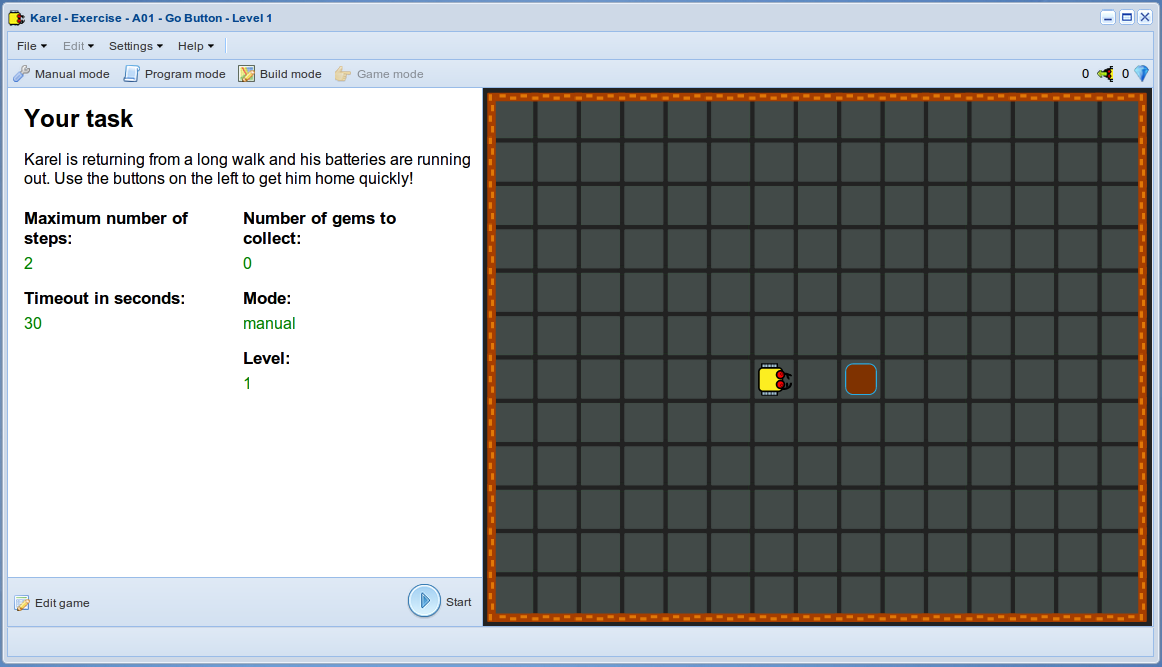
\includegraphics[width=0.7\textwidth]{img/a01.png}
\end{center}
\vspace{-4mm}
\caption{In the first game you need to help the robot get home}
\label{fig:a01}
\end{figure}
\noindent
Pressing Start will start 
the game, and at this time also the buttons Go, Turn, Get and Put appear, 
as shown in Fig. \ref{fig:a01b}.

\begin{figure}[!ht]
\begin{center}
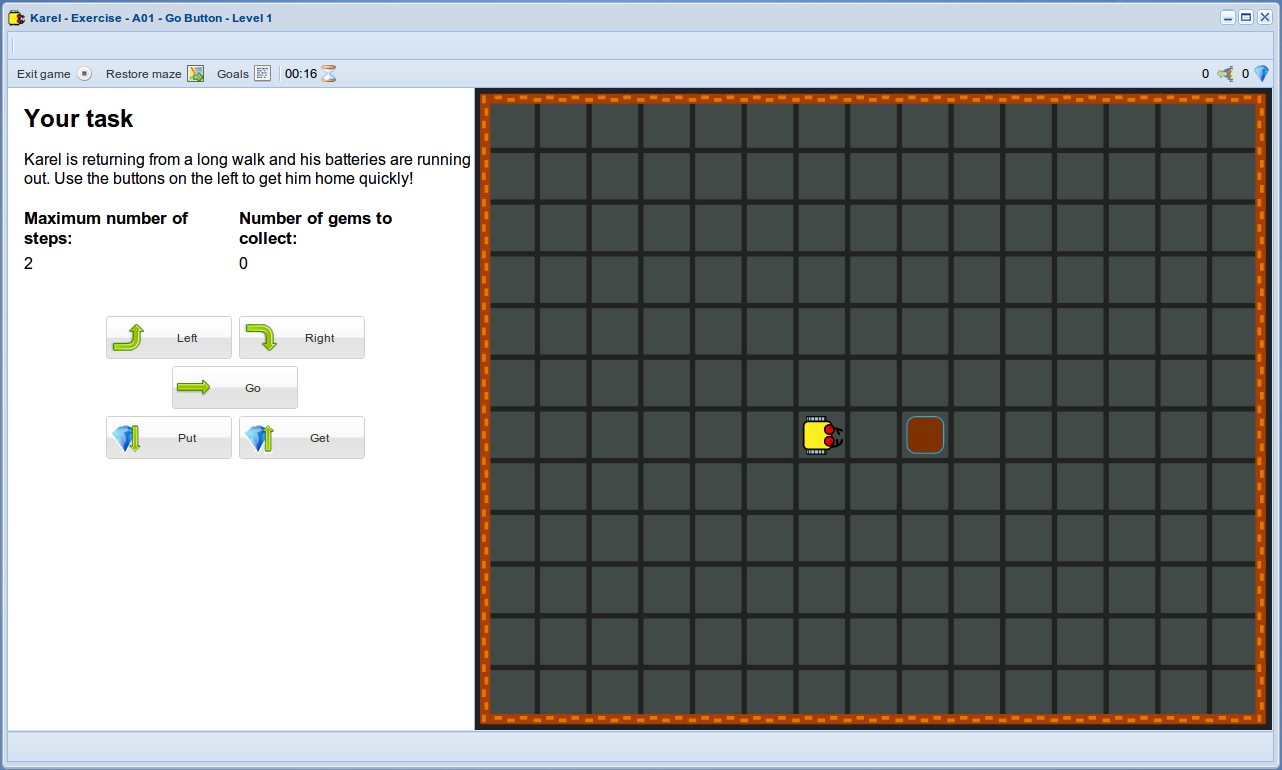
\includegraphics[width=0.7\textwidth]{img/a01b.png}
\end{center}
\vspace{-4mm}
\caption{Karel can be guided manually, using four buttons located in the left panel}
\label{fig:a01b}
\end{figure}

\newpage

\subsection{A02 - Olympic Games 1980}

{\em Karel is training for Robolympic Games! Your task is to run with 
the robot home as fast as possible. Karel's personal record is four seconds. How fast are you?}

\begin{figure}[!ht]
\begin{center}
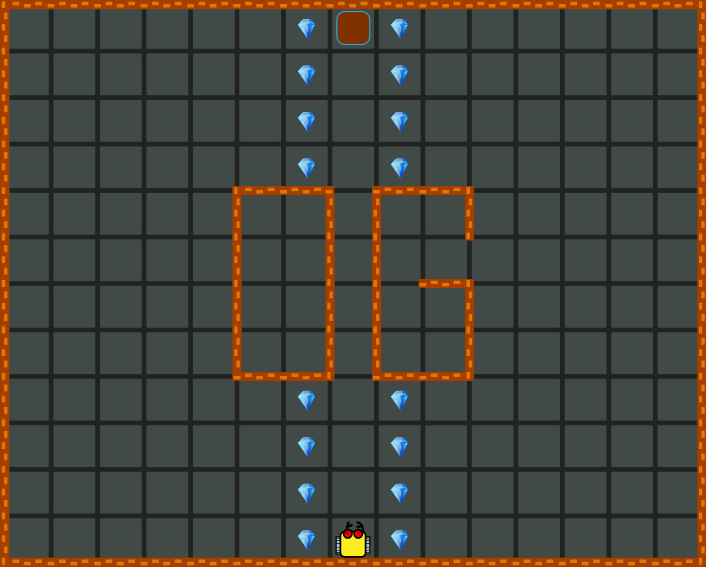
\includegraphics[width=0.7\textwidth]{img/a02.png}
\end{center}
\vspace{-4mm}
\caption{Karel is training for Robolympic Games}
\label{fig:a02}
\vspace{-4mm}
\end{figure}
\noindent

\subsection{A03 - Get Button}

{\em Today is Karel's lucky day because he is about to find his first gem. 
Use the buttons on the left to help the robot pick up the gem and carry it 
home!}

\begin{figure}[!ht]
\begin{center}
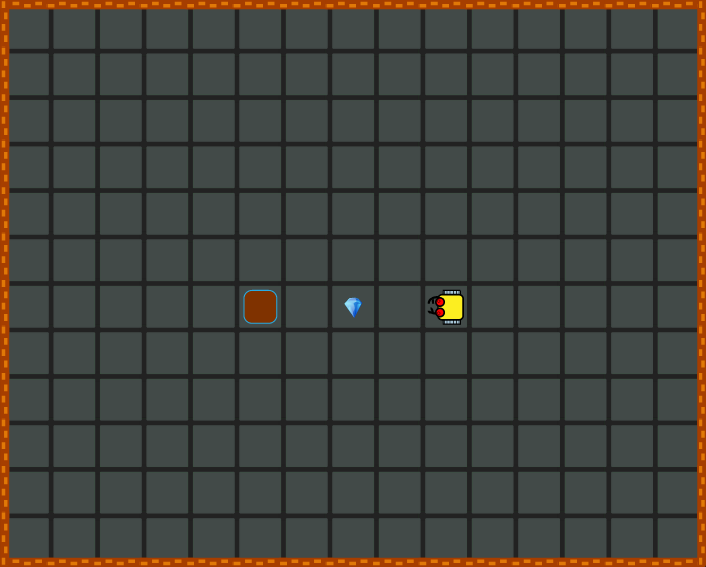
\includegraphics[width=0.7\textwidth]{img/a03.png}
\end{center}
\vspace{-4mm}
\caption{Karel is about to find his first gem}
\label{fig:a03}
\vspace{-1cm}
\end{figure}
\noindent
\newpage

\subsection{A04 - Olympic Games 1984}

{\em It is Robolympic season again! Run home as fast as you can, 
and collect all three gems on the way! Karel's personal record is 10 seconds.}

\begin{figure}[!ht]
\begin{center}
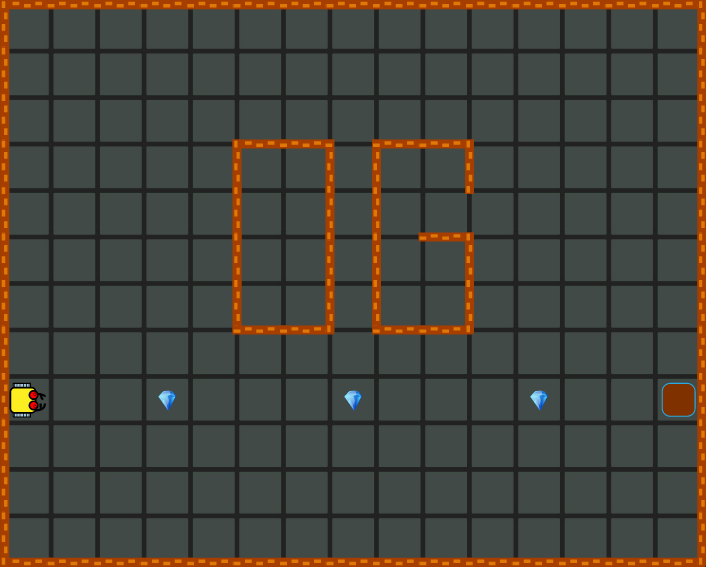
\includegraphics[width=0.7\textwidth]{img/a04.png}
\end{center}
\vspace{-4mm}
\caption{Karel's second Robolympic Games}
\label{fig:a04}
\end{figure}
\noindent


\subsection{A05 - Turn Button}

{\em Help the robot to collect the gem and return home!}

\begin{figure}[!ht]
\begin{center}
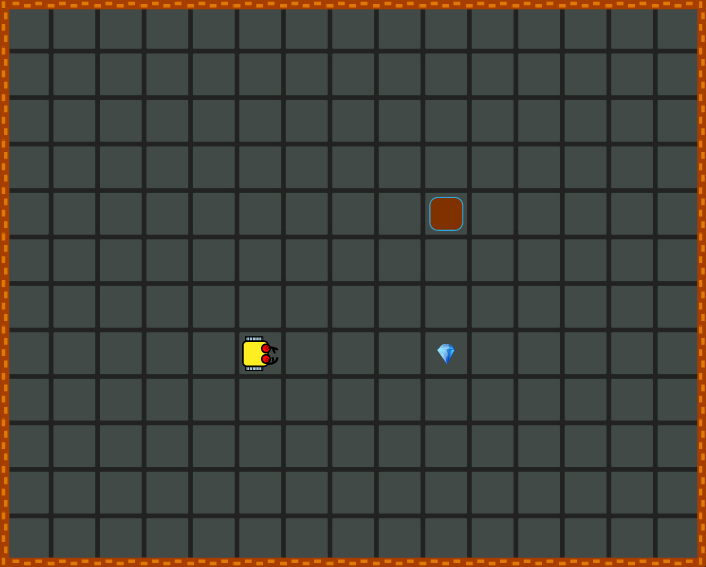
\includegraphics[width=0.7\textwidth]{img/a05.png}
\end{center}
\vspace{-4mm}
\caption{Karel is about to learn how to make a left turn}
\label{fig:a05}
\vspace{-1cm}
\end{figure}
\noindent
\newpage


\subsection{A06 - Olympic Games 1988 }

{\em Karel is training for his third Robolympic Games. Run with him around the block and home as fast as possible. He needs to collect at least one gem on the way. Karel's personal record is 16 seconds!}

\begin{figure}[!ht]
\begin{center}
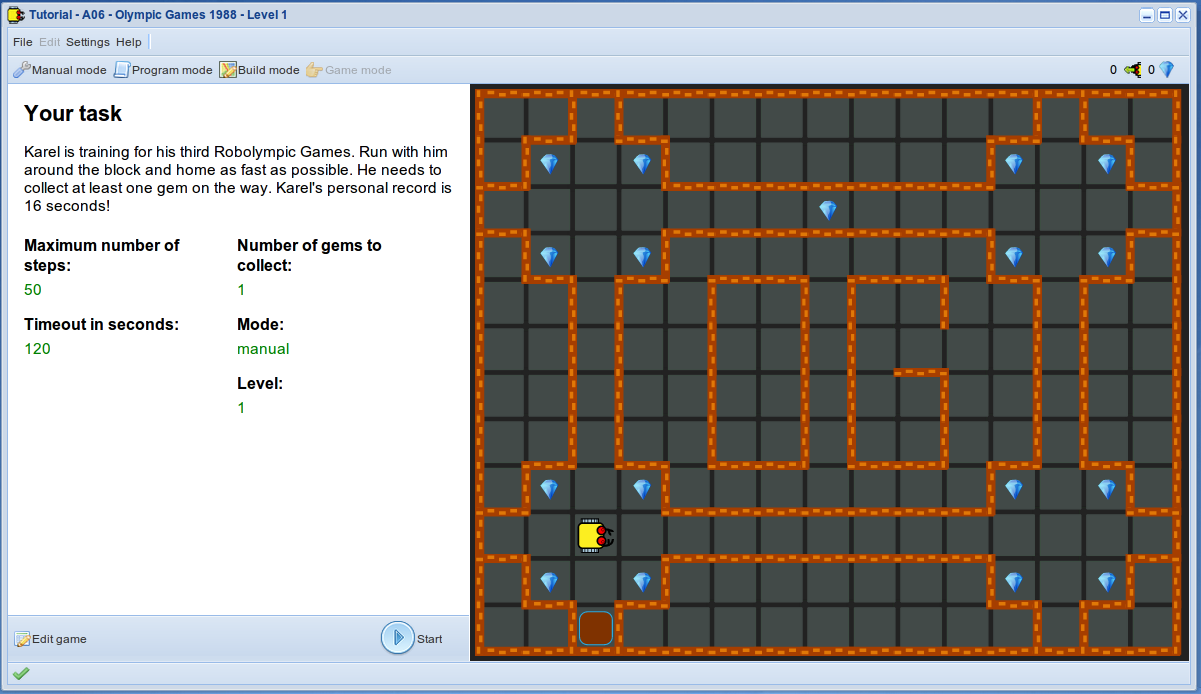
\includegraphics[width=0.7\textwidth]{img/a06.png}
\end{center}
\vspace{-4mm}
\caption{Karel's third Robolympic Games}
\label{fig:a06}
\end{figure}
\noindent


\subsection{A07 - Swirling Tornado}

{\em Pick up the two gems and get Karel home!}

\begin{figure}[!ht]
\begin{center}
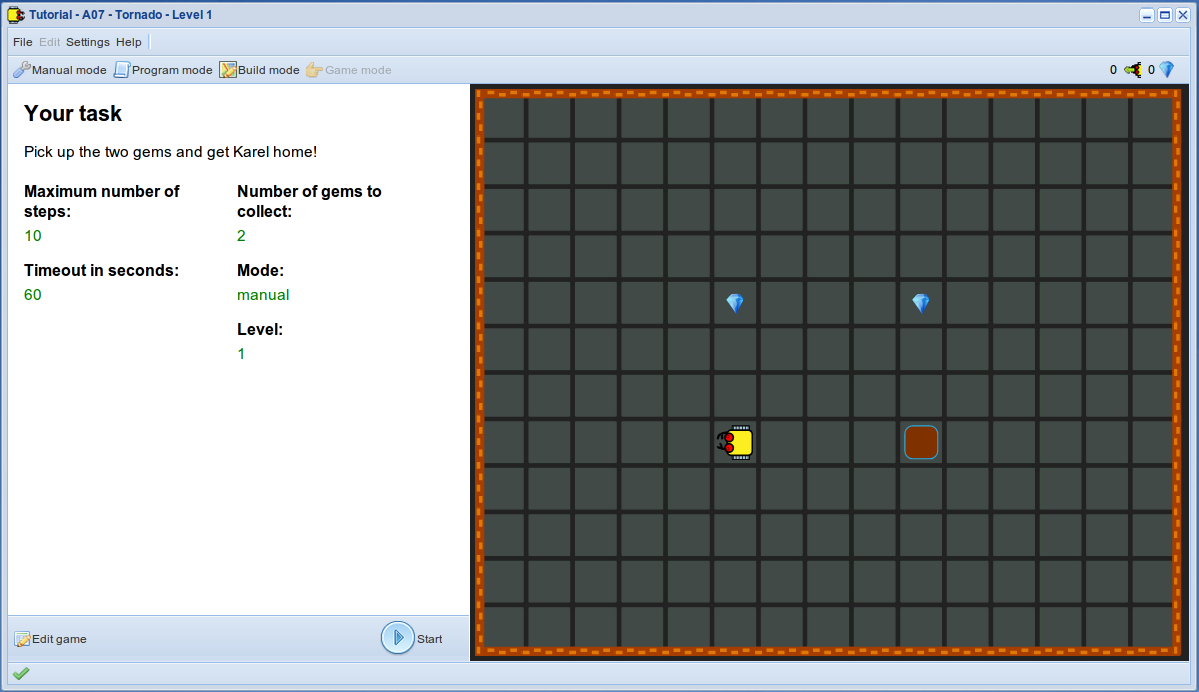
\includegraphics[width=0.7\textwidth]{img/a07.png}
\end{center}
\vspace{-4mm}
\caption{Karel will be swirling like a tornado}
\label{fig:a07}
\vspace{-1cm}
\end{figure}
\noindent
\newpage

\subsection{A08 - Olympic Games 1992}

{\em Last season of Karel's Robolympics Games is here! The 
robot needs to run home as fast as possible and bring one gem. 
Be careful not to crash, this is a tricky level! Karel's personal record is 26 seconds.}\\[-7mm]

\begin{figure}[!ht]
\begin{center}
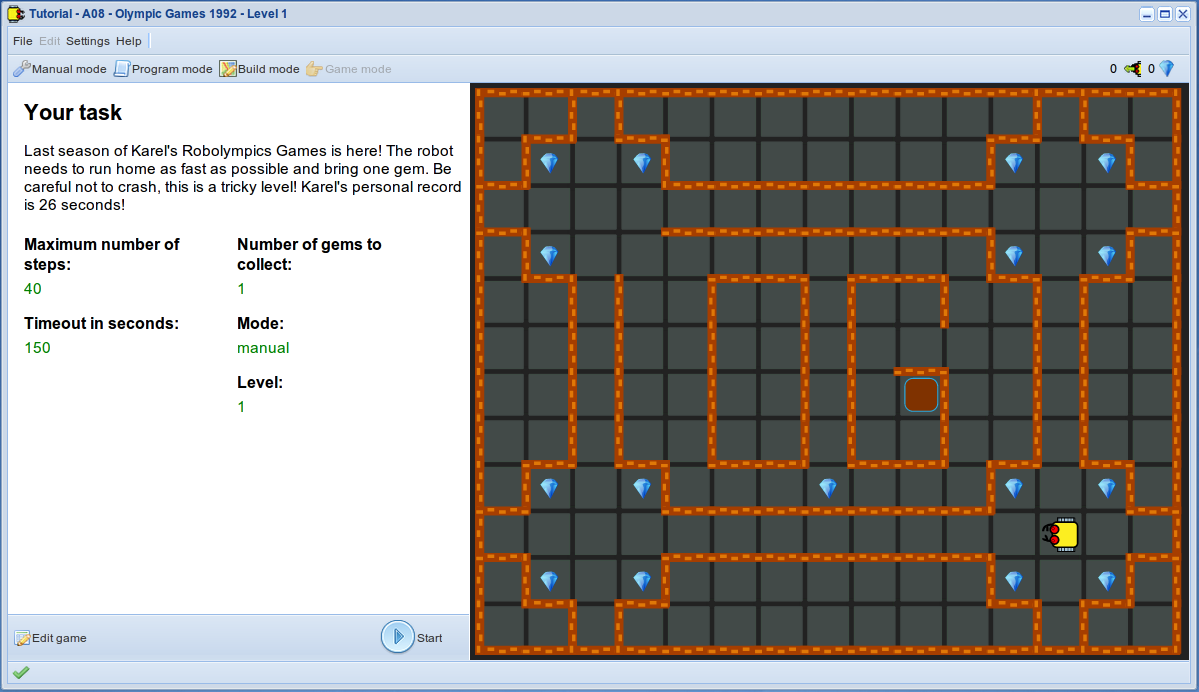
\includegraphics[width=0.7\textwidth]{img/a08.png}
\end{center}
\vspace{-4mm}
\caption{Karel's fourth Robolympic Games}
\label{fig:a08}
\vspace{-4mm}
\end{figure}
\noindent


\subsection{A09 - Maze Quest}

{\em This time Karel got seriously lost while looking for his favorite gem. 
Help him to collect the gem and find his way home!}\\[-7mm]

\begin{figure}[!ht]
\begin{center}
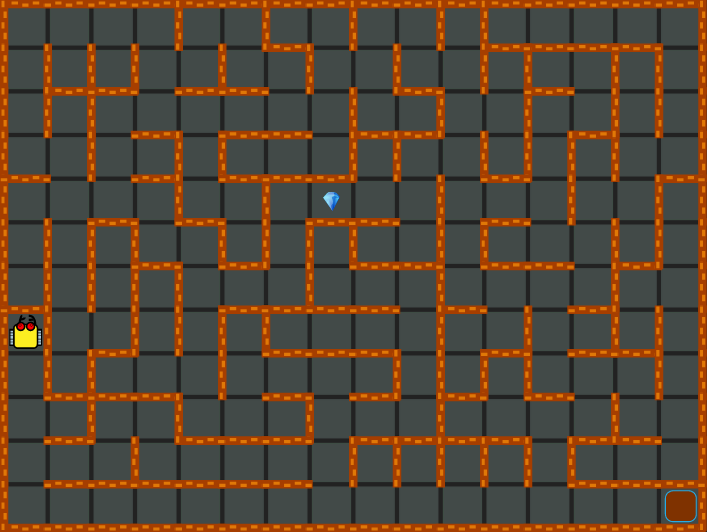
\includegraphics[width=0.7\textwidth]{img/a09.png}
\end{center}
\vspace{-4mm}
\caption{Karel got lost while looking for his favorite gem}
\label{fig:a09}
\vspace{-4mm}
\end{figure}
\noindent
\newpage

\subsection{A10 - Labyrinth}

{\em This is a true labyrinth and your task is to lead Karel 
home. Remember - think first before going anywhere!}

\begin{figure}[!ht]
\begin{center}
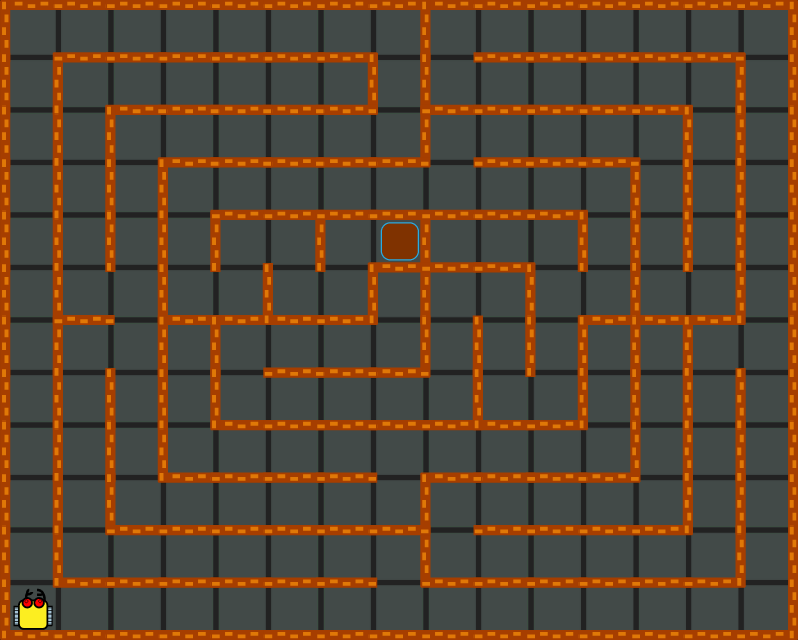
\includegraphics[width=0.7\textwidth]{img/a10.png}
\end{center}
\vspace{-4mm}
\caption{Karel needs to find his way home in a labyrinth}
\label{fig:a10}
\vspace{-4mm}
\end{figure}
\noindent


\subsection{A11 - Diamond Mine}

{\em Karel discovered an abandoned diamond mine. Use the buttons
on the left to collect all gems and get back home in time!}

\begin{figure}[!ht]
\begin{center}
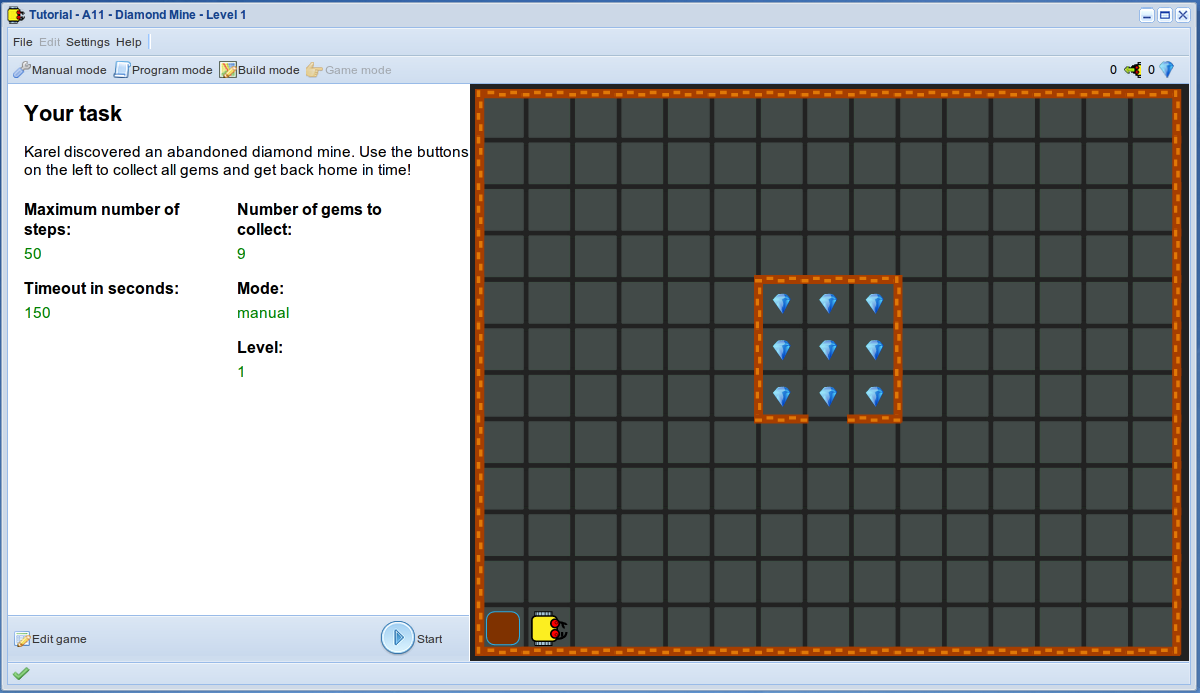
\includegraphics[width=0.7\textwidth]{img/a11.png}
\end{center}
\vspace{-4mm}
\caption{Karel found an abandoned diamond mine}
\label{fig:a11}
\vspace{-4mm}
\end{figure}
\noindent
\newpage

\subsection{A12 - Gem Harvest}

{\em If gems are piled up, then a number is showing their amount. 
Help Karel collect all gems in this maze and return home!}\\[-7mm]

\begin{figure}[!ht]
\begin{center}
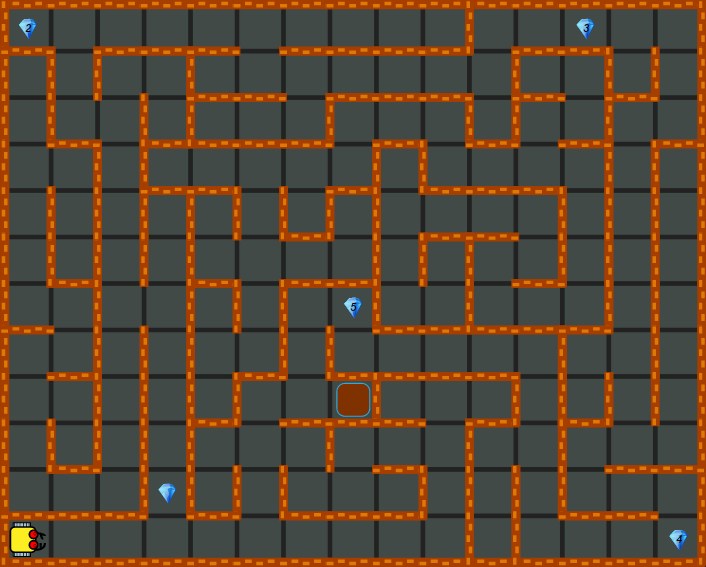
\includegraphics[width=0.7\textwidth]{img/a12.png}
\end{center}
\vspace{-4mm}
\caption{If gems are piled up, then a number is showing their amount}
\label{fig:a12}
\vspace{-4mm}
\end{figure}
\noindent


\subsection{A13 - Put Button}

{\em Karel has five gems in his bag. Use the buttons on the left to put the gems on the table and 
return home in time!}\\[-7mm]

\begin{figure}[!ht]
\begin{center}
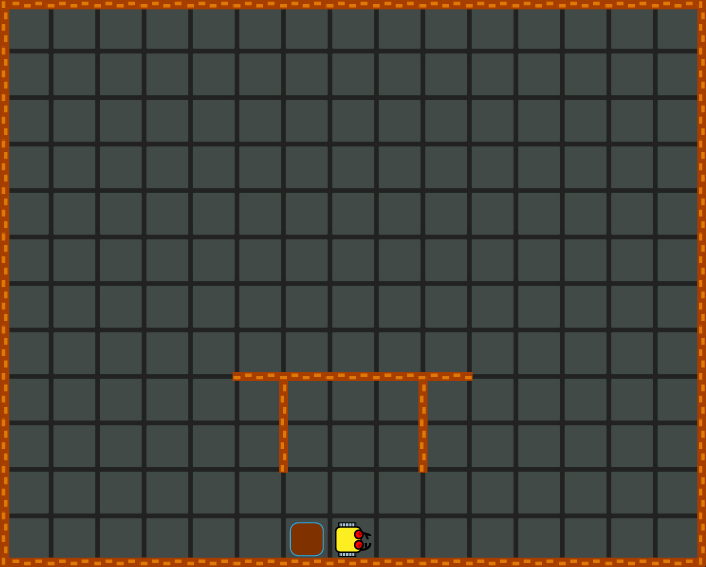
\includegraphics[width=0.7\textwidth]{img/a13.png}
\end{center}
\vspace{-4mm}
\caption{Karel needs to put five gems on the table}
\label{fig:a13}
\vspace{-4mm}
\end{figure}
\noindent
\newpage

\section{Lesson Two - Taking the Leap}

In this Lesson you will help Karel solve tasks again,
but no longer using the mouse. From now on you will be 
typing commands {\tt go}, {\tt get}, {\tt turn} and {\tt put} 
instead of pressing the buttons Go, Get, Turn and Put. The 
commands do exactly the same things as the corresponding buttons.  
There are only two new rules to remember:
\begin{enumerate} 
\item Type the commands into the input cell on the left, always one command per line.
\item The program is run by clicking on the "Run program" button in the menu, or by clicking 
      on the link "run" under the input cell.
\end{enumerate}
You can clone all games in this Lesson into your account via the File Manager's Project
menu, same as you did with the games in Lesson 1, and moreover you can clone their solutions. 
Solution manual in PDF is also provided. 

\subsection{B01 - Go Command}

{\em Write a program that gets Karel home! Remember: Typing "go" is exactly 
the same as pressing the Go button. Always write one command per line.}

\begin{figure}[!ht]
\begin{center}
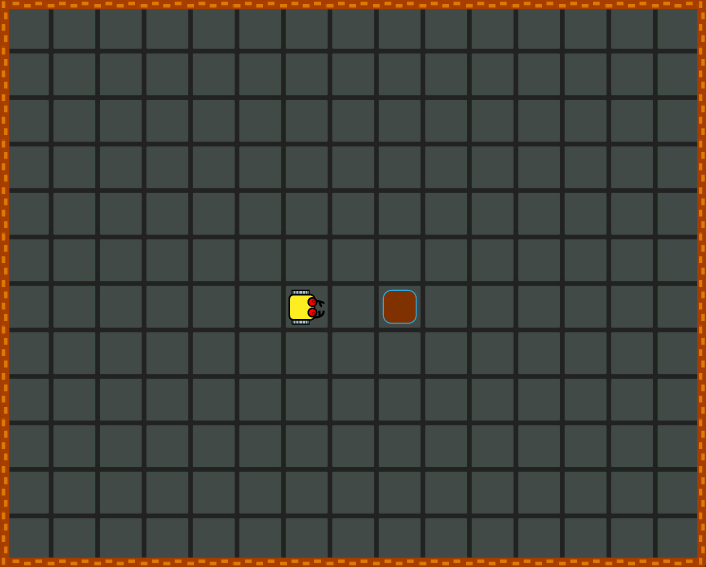
\includegraphics[width=0.7\textwidth]{img/b01.png}
\end{center}
\vspace{-4mm}
\caption{Get Karel home using the {\tt go} command}
\label{fig:b01}
\vspace{-4mm}
\end{figure}
\noindent

\newpage
\subsection{B02 - Get Command}

{\em Write a program for Karel to collect all gems and get home! 
Remember that typing "get" is the same as pressing the Get button.}\\[-7mm]

\begin{figure}[!ht]
\begin{center}
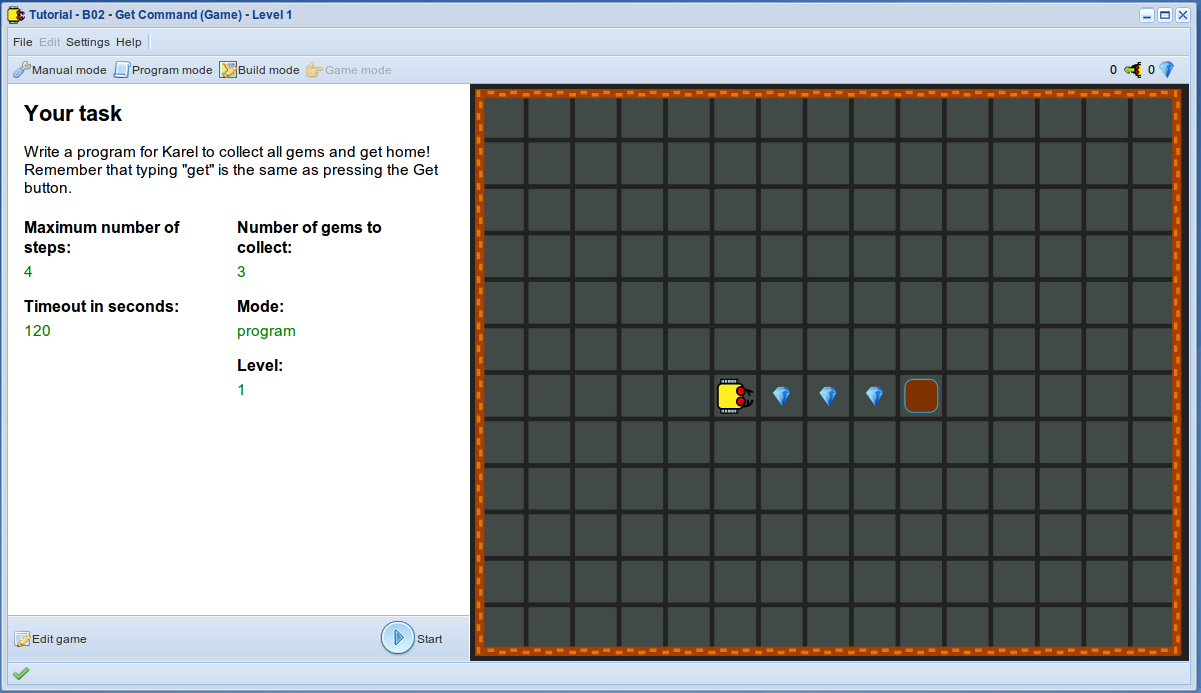
\includegraphics[width=0.7\textwidth]{img/b02.png}
\end{center}
\vspace{-4mm}
\caption{Collecting gems via the {\tt get} command}
\label{fig:b02}
\vspace{-4mm}
\end{figure}
\noindent

\subsection{B03 - Turn Command}

{\em Write a program for Karel to collect the gem and return 
home! Remember: Typing "turn" is exactly the same as pressing 
the Turn button.}\\[-7mm]

\begin{figure}[!ht]
\begin{center}
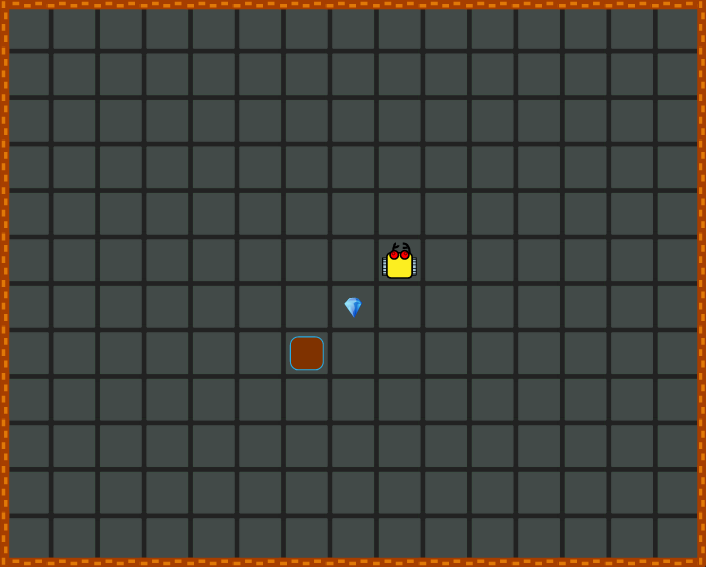
\includegraphics[width=0.7\textwidth]{img/b03.png}
\end{center}
\vspace{-4mm}
\caption{Navigating to the left and to the right via the {\tt turn} command}
\label{fig:b03}
\vspace{-4mm}
\end{figure}
\noindent
\newpage

\subsection{B04 - Put Command}

{\em Write a program for Karel to pick up the gem, turn around, make 
two steps, put the gem on the ground, and return home! Remember: 
Writing "put" is exactly the same as pressing the Put button.}

\begin{figure}[!ht]
\begin{center}
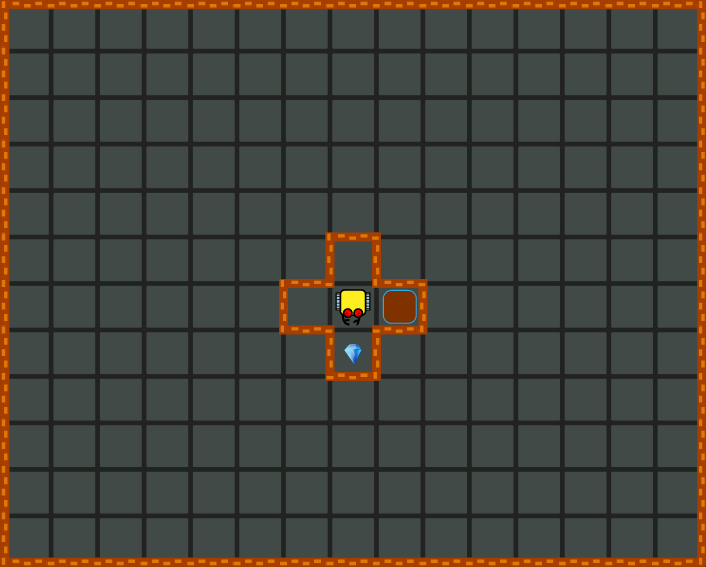
\includegraphics[width=0.7\textwidth]{img/b04.png}
\end{center}
\vspace{-4mm}
\caption{Karel moves a gem from one corner to another using the {\tt put} command}
\label{fig:b04}
\vspace{-4mm}
\end{figure}
\noindent


\section{Lesson Three - Making It Short and Elegant}

In Lesson Two you learned that Karel accepts commands and that he always obeys 
them exactly. Sometimes even {\em too exactly}, meaning that you may have planned
something different from what the robot actually did. Do not worry about that, this
is happening all the time and even to the greatest programmers. But it helps to be careful and 
think twice before writing a program. You have to go in your mind through 
all the commands that you want the robot to follow. You have to play the program 
in your head, then the robot will do exactly what you want him to do. 

This Lesson will teach you a simple and elegant way to save lots of typing 
by using the {\tt repeat} command. It is very simple. Imagine that you want the
robot to turn to the right. To do this, he needs to turn three times to the left:

\begin{verbatim}
turn
turn
turn
\end{verbatim}
But the same can be achieved by telling Karel to {\tt repeat} the {\tt turn} command {\tt 3} times:

\begin{verbatim}
repeat 3
  turn
\end{verbatim}
Notice that the command {\tt turn} is indented by two characters. This is important
because it means that the command {\tt turn} is in the {\em body} of the {\tt repeat} 
command. If we want to repeat multiple commands, then all of them need to be indented. 
For example, to repeat {\tt go} and {\tt turn} three times, we type:

\begin{verbatim}
repeat 3
  go
  turn
\end{verbatim}
That's it! Enough of studying, now let's go play some computer
games. As before, you can clone all of them via the File Manager's Project menu.

 
\subsection{C01 - Ten Steps}

{\em Karel's home is ten steps away, so you could type "go" ten times to get him home. 
However, your task is to write a program that has only \underline{two lines}. Remember, we always 
write one command per line.}

\begin{figure}[!ht]
\begin{center}
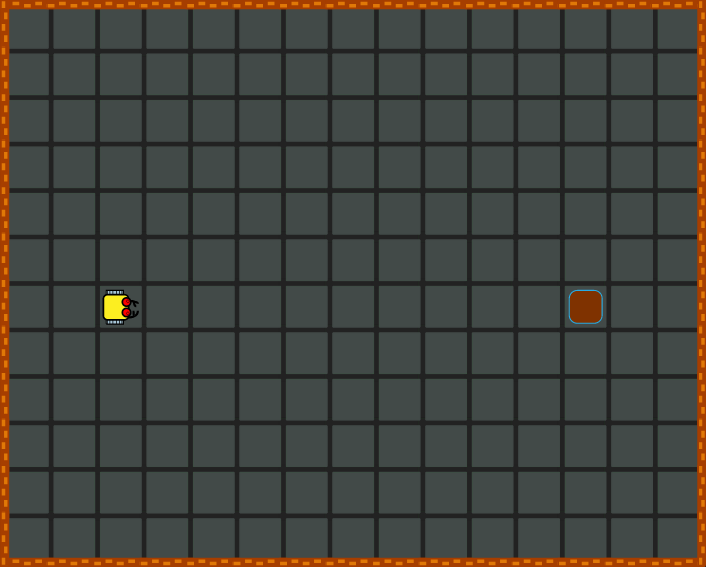
\includegraphics[width=0.7\textwidth]{img/c01.png}
\end{center}
\vspace{-4mm}
\caption{Karel gets home elegantly, using the {\tt repeat} command}
\label{fig:c01}
\vspace{-4mm}
\end{figure}
\noindent

\newpage

\subsection{C02 - Nine Gems}

{\em Write a program for Karel to collect all nine gems and get home! 
Writing one command per line, your program should not have more 
than \underline{three lines}}.

\begin{figure}[!ht]
\begin{center}
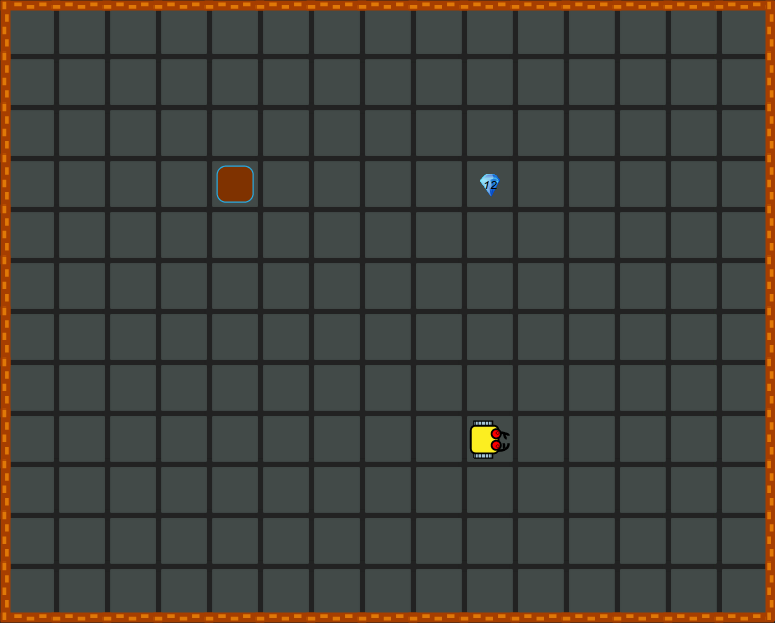
\includegraphics[width=0.7\textwidth]{img/c02.png}
\end{center}
\vspace{-4mm}
\caption{Nine gems are between Karel and his home}
\label{fig:c02}
\vspace{-4mm}
\end{figure}
\noindent


\subsection{C03 - Diamond Staircase}

{\em Write a program for Karel to collect all gems and get home! 
With one command per line, your program should be no longer than \underline{7 lines}.}

\begin{figure}[!ht]
\begin{center}
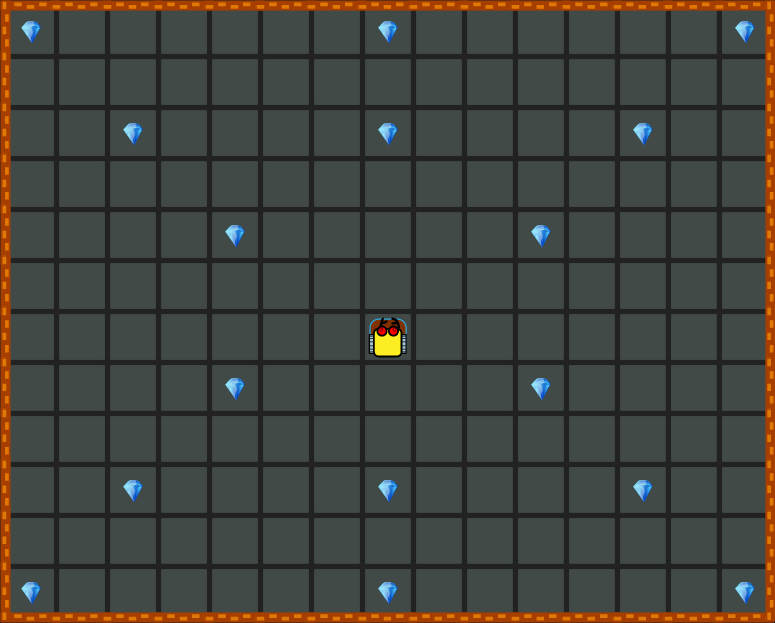
\includegraphics[width=0.7\textwidth]{img/c03.png}
\end{center}
\vspace{-4mm}
\caption{This time Karel has to do some climbing}
\label{fig:c03}
\vspace{-4mm}
\end{figure}
\noindent

\newpage

\subsection{C04 - Nesting}

{\em In programming, it is of essence to recognize repeating patterns. 
Write a program for Karel to collect all gems and get back home! With 
one command per line, your program should have at most \underline{5 lines}.
Hint: you may want to use a {\tt repeat} command in the body of another
{\tt repeat} command - this is called {\em nesting}.}

\begin{figure}[!ht]
\begin{center}
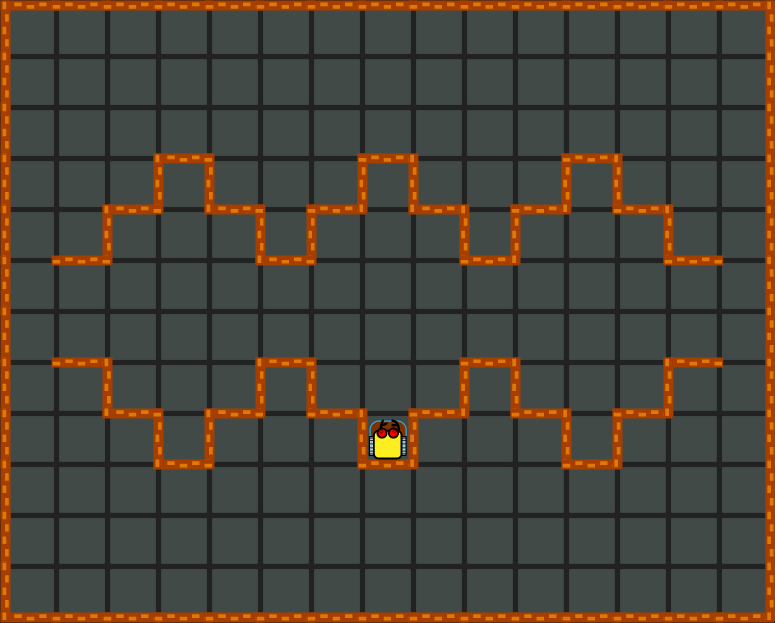
\includegraphics[width=0.7\textwidth]{img/c04.png}
\end{center}
\vspace{-4mm}
\caption{This time Karel will need two nested {\tt repeat} commands}
\label{fig:c04}
\vspace{-4mm}
\end{figure}
\noindent



\section{Lesson Four - Using Sensors}

Karel has five built-in sensors to better navigate in the maze. 
The first one is an infrared sensor that the robot uses to determine 
whether it is safe to move forward, or whether there is a wall ahead.
The usage can be illustrated on a simple program "Careful step" 
where Karel first checks whether there is a wall ahead before
making a step. If there is wall, he does not crash into it but turns 
back instead: 

\begin{verbatim}
# Program "Careful step".
if wall
  turn
  turn
else
  go
\end{verbatim}
Note that the symbol {\tt \#} introduces a comment, meaning that the line 
of code behind it is ignored by the robot.
The {\tt else} branch does not have to be there. Notice the indentation 
of the bodies of the {\tt if} and {\tt else} branches - this is analogous 
to how we indented the body of the {\tt repeat} command.

Besides {\tt wall}, the robot can check the following:
\begin{itemize}
\item {\tt gem} ... is there a gem where he stands?
\item {\tt empty} ... is his bag with gems empty?
\item {\tt north} ... is he facing North?
\item {\tt home} ... is he at home?
\end{itemize}
Karel can also use the reserved word {\tt not} to test the opposites.
For illustration, the previous program can be rewritten as follows, without changing its function:
\begin{verbatim}
# Program "Careful step".
if not wall
  go
else
  turn
  turn
\end{verbatim}
BEWARE -- if you crash the robot into a wall, if you ask him to collect a gem where there
is none, or if you ask him to put a gem on the ground while 
his bag is empty, {\bf he will throw an error.}. Throwing an error 
means to say something impolite and go on strike!\\

\noindent
Now let's go play some games.

\subsection{D01 - Foggy Road}

{\em Several gems lie on the ground between the robot and his home which is 10 steps away. 
He cannot see where they are exactly since his sensor only tells him if a gem is right 
under him.  And besides that, nothing is visible in today's foggy weather anyway. 
Write a program for Karel to collect all gems and get home. With one command per 
line, your program should have at most \underline{4 lines}.}

\newpage

\begin{figure}[!ht]
\begin{center}
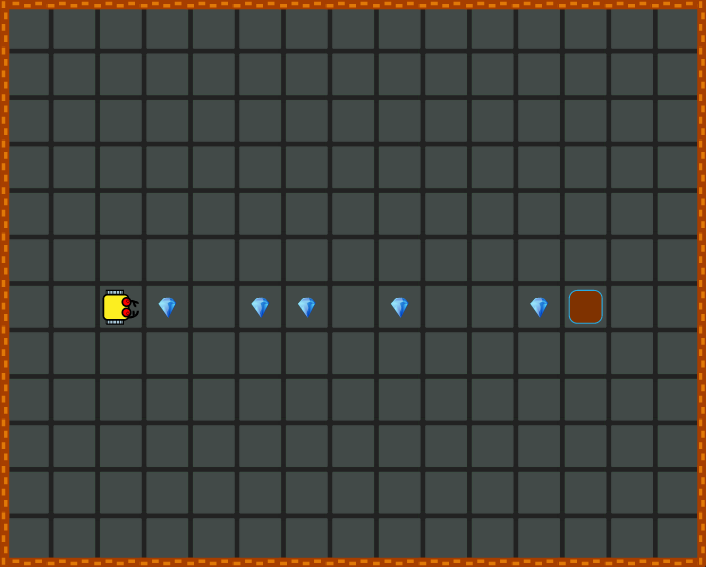
\includegraphics[width=0.7\textwidth]{img/d01.png}
\end{center}
\vspace{-4mm}
\caption{Collecting gems along a foggy road}
\label{fig:d01}
\vspace{-4mm}
\end{figure}
\noindent



\subsection{D02 - Secret Chest}

{\em Karel stores all his gems in a secret chest in his cellar. 
Currently, some shelves are empty. Write a program for Karel to 
inspect all shelves and put a gem where one is missing! After that, he needs to get 
home as usual With one 
command per line, your program should have at most \underline{7 lines}.}

\begin{figure}[!ht]
\begin{center}
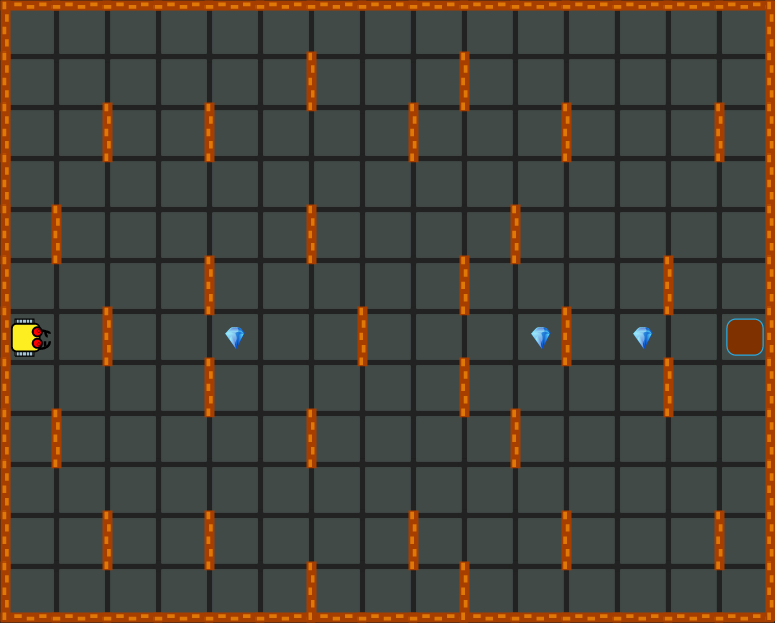
\includegraphics[width=0.7\textwidth]{img/d02.png}
\end{center}
\vspace{-4mm}
\caption{Filling his secret chest with gems}
\label{fig:d02}
\vspace{-4mm}
\end{figure}
\noindent



\section{Lesson Five - The Smart Loop}

Sometimes Karel needs to repeat something even though he does not know 
the number of repetitions a-priori. This can be the case, for example, 
when he is asked to walk straight ahead until he reaches the closest wall:

\begin{verbatim}
while not wall
  go
\end{verbatim}
Or, he may be asked to walk until he gets home:

\begin{verbatim}
while not home
  go
\end{verbatim}
Or, he may be asked to empty his bag although he does not know how 
many gems are in it: 
 
\begin{verbatim}
while not empty
  put
\end{verbatim}
Or, he may be asked to collect all gems from a pile although he does
not know how many gems there are:

\begin{verbatim}
while gem
  get
\end{verbatim}
Or, to give a last example, we may ask him to turn to face North, 
although he does not know at the moment which direction he is
facing:

\begin{verbatim}
while not north
  turn
\end{verbatim}
Just for fun, let us introduce one more example where Karel is asked to 
turn South, walk straight ahead until he reaches the closest wall, and 
collect all gems that he can find on the way:

{\small
\begin{verbatim}
# First turn south.
while not north
  turn
repeat 2
  turn
# Go straight ahead and pick all gems.
while not wall
  if gem
    get
  go
# Pick gem at the wall if any.
if gem
  get
\end{verbatim}
}

\newpage
\subsection{E01 - Looking for Home}

{\em Karel knows that his home is straight ahead, but he does not know how far - he does not 
have any sensor that would tell him. 
Write a program to get him there safely! Your program should only have \underline{2 lines}.}\\[-7mm]

\begin{figure}[!ht]
\begin{center}
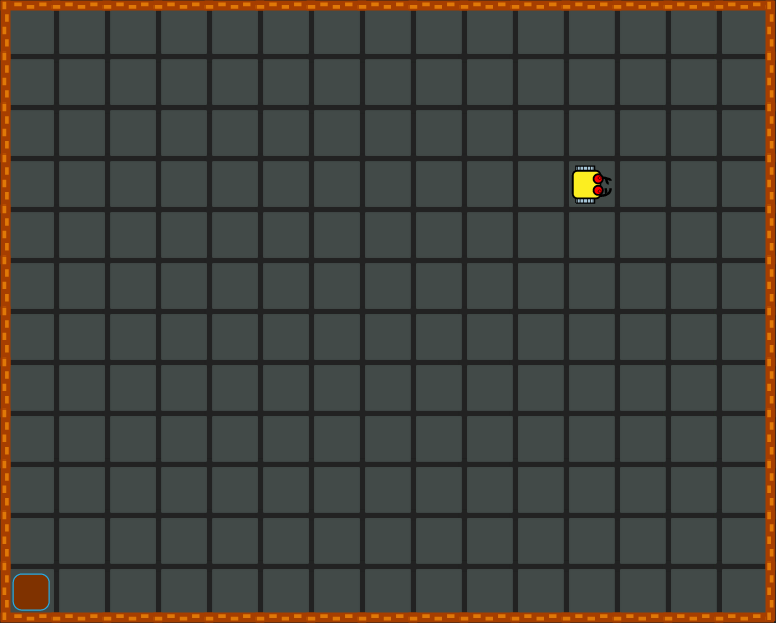
\includegraphics[width=0.7\textwidth]{img/e01.png}
\end{center}
\vspace{-4mm}
\caption{Karel does not know how far from home he is}
\label{fig:e01}
\vspace{-12mm}
\end{figure}
\noindent


\subsection{E02 - Hide-and-Seek}

{\em Karel's friends are hiding. He knows that he has to go straight 
ahead to find them. When he finds a gem, he has to turn left and keep 
walking. Eventually, he will get to the place where his friends are 
hiding. If he gets home, stop. Write a program for Karel to do this, 
and do not forget to collect all the gems on the way!}\\[-7mm]

\begin{figure}[!ht]
\begin{center}
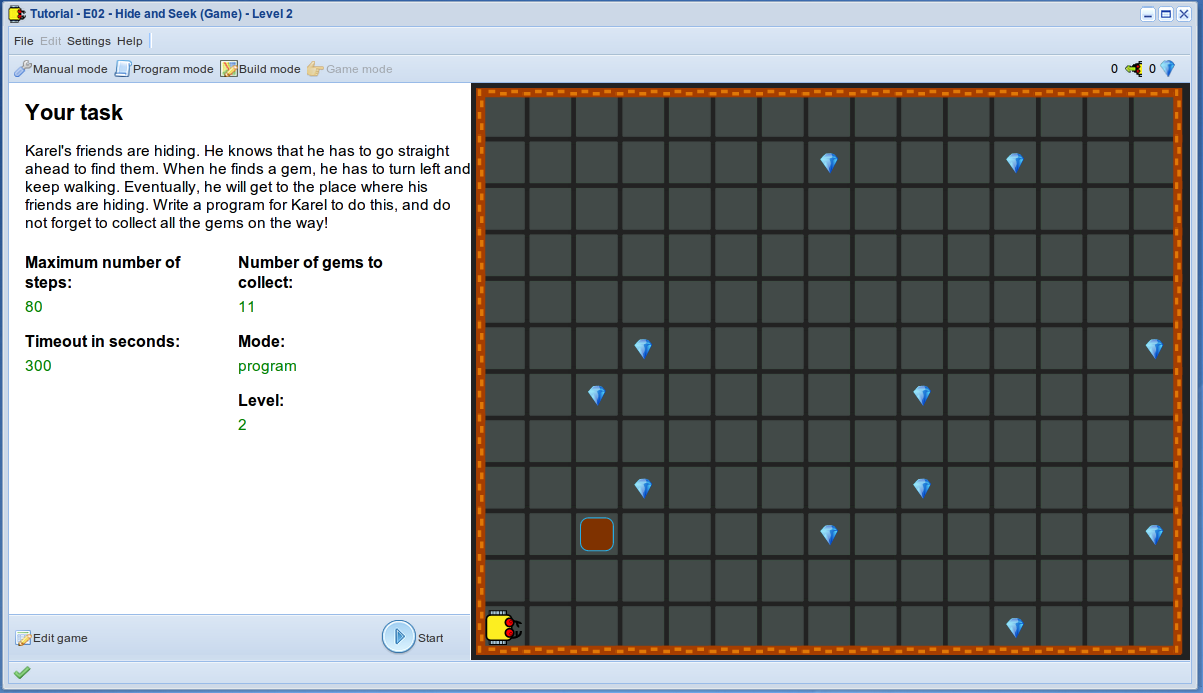
\includegraphics[width=0.7\textwidth]{img/e02.png}
\end{center}
\vspace{-4mm}
\caption{Karel plays hide-and-seek with his friends}
\label{fig:e02}
\vspace{-10mm}
\end{figure}
\noindent
\newpage

\section{Lesson Six - Keeping It Simple}

{\bf Keeping it simple is the most important thing of all in programming.} 
Always look for small tasks that are repeated thoroughout the 
solution of the big task. Solve the small tasks first, and you'll
see that the big task gets simpler. The importance of what we
just said cannot be stressed more. Please read it once more.\\

\noindent
The fact that you are reading this line of text proves that you are not a Robot.
Otherwise you would be stuck forever in the previous paragraph which is 
an infinite loop!\\

\noindent
New commands for simpler tasks are defined using the reserved word 
{\tt def}. For example, in a program where the robot needs to turn to the 
right many times, it is a good idea to define a new command {\tt turn\_right}
as follows:

\begin{verbatim}
def turn_right
  repeat 3
    turn
\end{verbatim}
To illustrate this, let's return to the game A07 - Swirling Tornado.
A really bad program to solve this task would be:

{\small
\begin{verbatim}
turn
turn
turn
go
go
go
go 
get
turn
turn
turn
go
go
go
go 
get
turn
turn
turn
go
go
go
go
get
\end{verbatim}
}
\noindent
Can you see how many times the same code is repeated?! In order to fix this, 
we should define new commands {\tt right\_turn} and {\tt four\_steps} as
follows:

{\small
\begin{verbatim}
def right_turn
  repeat 3
    turn

def four_steps
  repeat 4
    go
\end{verbatim}
}
\noindent
With these two new commands, the above code simplifies to 

{\small
\begin{verbatim}
right_turn
four_steps
get
right_turn
four_steps
get
right_turn
four_steps
get
\end{verbatim}
}
\noindent
There are still repetitions that must be eliminated! So we define a new command 
{\tt walk\_edge}:

{\small
\begin{verbatim}
def walk_edge
  right_turn
  four_steps
  get
\end{verbatim}
}
\noindent
Now with the three new commands {\tt right\_turn}, {\tt four\_steps} and
{\tt walk\_edge}, our program simplifies to:

{\small
\begin{verbatim}
while not home
  walk_edge
\end{verbatim}
}
\noindent
It is the task of the first game in this Lesson to implement this program. But before we 
do so, let us mention one very important thing.

\subsection{Solution procedure revisited (and corrected)}


An experienced programmer would never solve the problem the way we did.
He would first look at the problem, trying to recognize repeating patterns. 
He would find that the task can be fulfilled by repeating one simpler task 
three times. So, without knowing exactly how the smaller task is going to 
be solved, he would write:

{\small
\begin{verbatim}
while not home
  walk_edge
\end{verbatim}
}
\noindent
Next he would define the new command {\tt walk\_edge} as follows:

{\small
\begin{verbatim}
def walk_edge
  right_turn
  four_steps
  get
\end{verbatim}
}
\noindent
He would not bother yet defining the commands {\tt right\_turn} and 
{\tt four\_steps} exactly, because he knows that this will be very 
simple. And as the last step, to make the program work, he would 
define:

{\small
\begin{verbatim}
def right_turn
  repeat 3
    turn

def four_steps
  repeat 4
    go
\end{verbatim}
}
\noindent
Keep this in mind while solving the following games!


\subsection{F01 - Swirling Tornado is Back}

{\em Write a program for Karel to pick up the two gems and get home! }

\begin{figure}[!ht]
\begin{center}
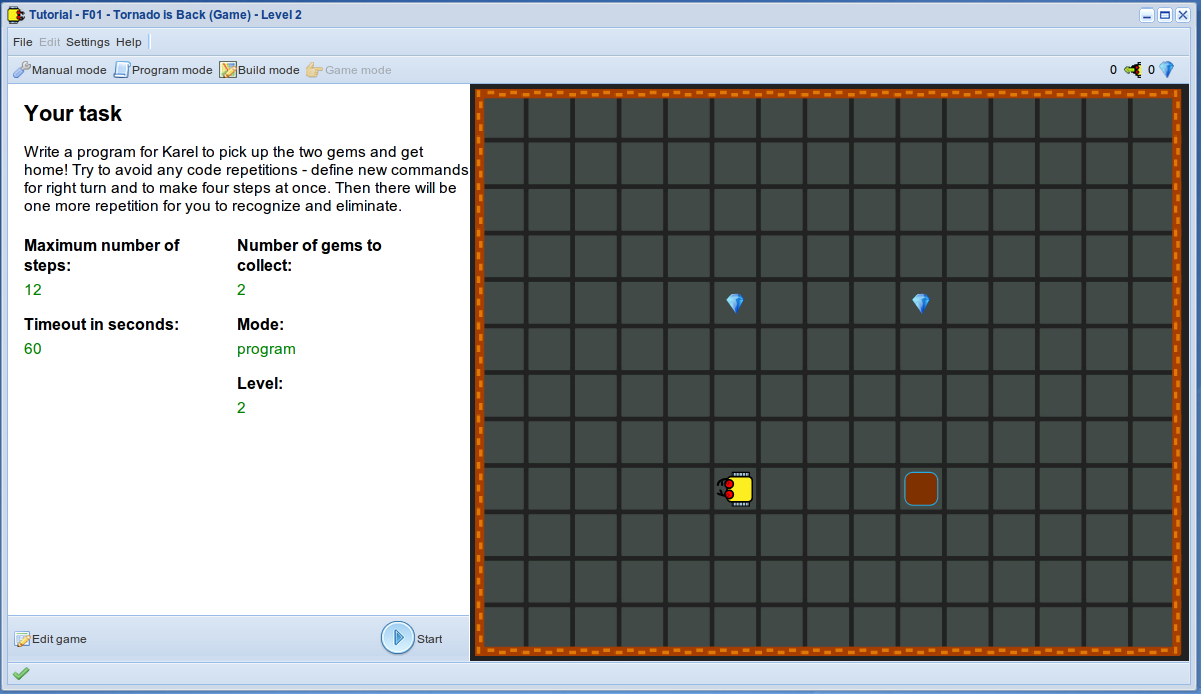
\includegraphics[width=0.7\textwidth]{img/f01.png}
\end{center}
\vspace{-4mm}
\caption{Solving the Swirling Tornado problem again, now as a Programmer}
\label{fig:f01}
\vspace{-10mm}
\end{figure}
\noindent
\newpage


\subsection{F02 - Diamond Staircase is Back}

{\em Write a program for Karel to collect all gems and get home! 
Now, being an experienced programmer, first identify the repeating 
pattern and define a new command for the simpler task. Write the main 
program using this new command. Then as the last step, define the 
details of the new command.}\\[-7mm]

\begin{figure}[!ht]
\begin{center}
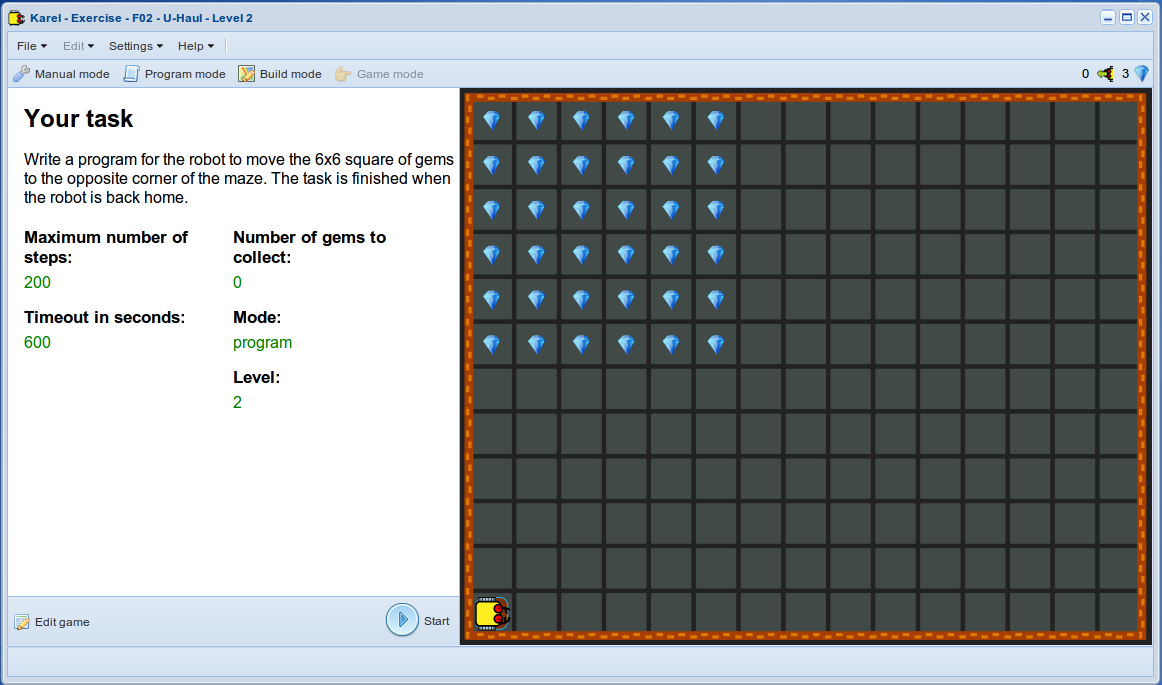
\includegraphics[width=0.7\textwidth]{img/f02.png}
\end{center}
\vspace{-4mm}
\caption{Solving the Diamond Staircase again, now as a Programmer}
\label{fig:f02}
\vspace{-10mm}
\end{figure}
\noindent

\subsection{F03 - Pirate Ship}

{\em Karel is on a pirate ship! Write a program for him to collect all 
gems and run away (to his home) before the pirates are back. Here Karel 
needs to be extremely efficient to survive. Therefore, there should be 
no repeating parts whatsoever in your program!}\\[-7mm]


\begin{figure}[!ht]
\begin{center}
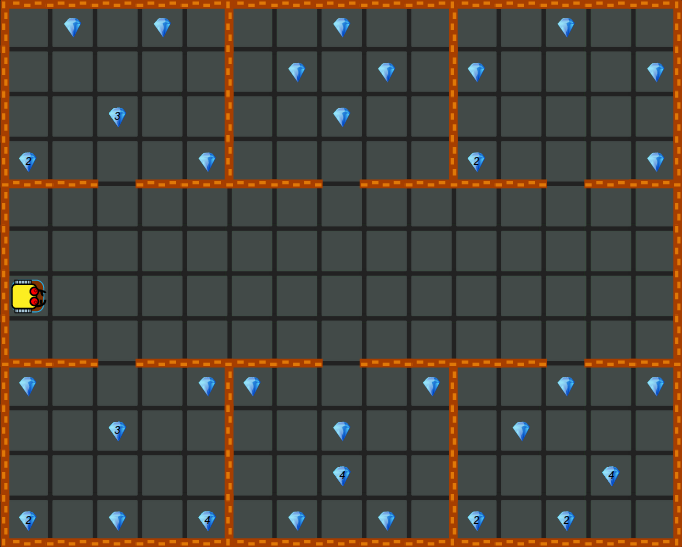
\includegraphics[width=0.7\textwidth]{img/f03.png}
\end{center}
\vspace{-4mm}
\caption{Karel found a pirate treasure}
\label{fig:f03}
\vspace{-10mm}
\end{figure}
\noindent

\newpage

\section{More Games!}

All games in this section can be cloned via the File Manager's
Project menu. Some of them come with solutions, some others 
are still waiting for their solution to be published.

\subsection{Easy - Easy Pick}

{\em Write a program to get Karel home, collecting all the 
gems he can find. The gems are randomly distributed, so 
you cannot use their exact positions in your program!
}

\begin{figure}[!ht]
\begin{center}
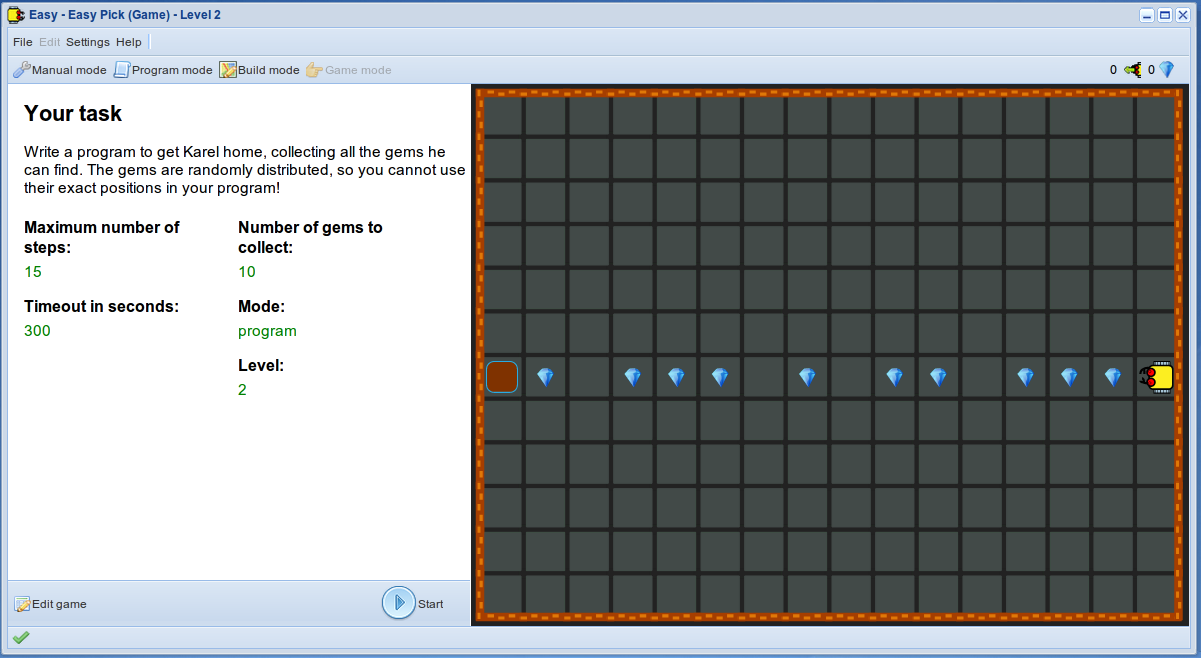
\includegraphics[width=0.7\textwidth]{img/game-easypick.png}
\end{center}
\vspace{-4mm}
\caption{Picking these gems is so easy!}
\label{fig:easypick}
\vspace{-10mm}
\end{figure}
\noindent

\newpage
\subsection{Easy - Gem Jam!}

{\em In this maze, gems are distributed randomly along the walls. Otherwise 
the maze is empty. Karel's home is in the south-west corner, and the robot 
stands on the right of it, facing east. Write a program for Karel to collect 
all the gems and return home. Good luck!  }

\begin{figure}[!ht]
\begin{center}
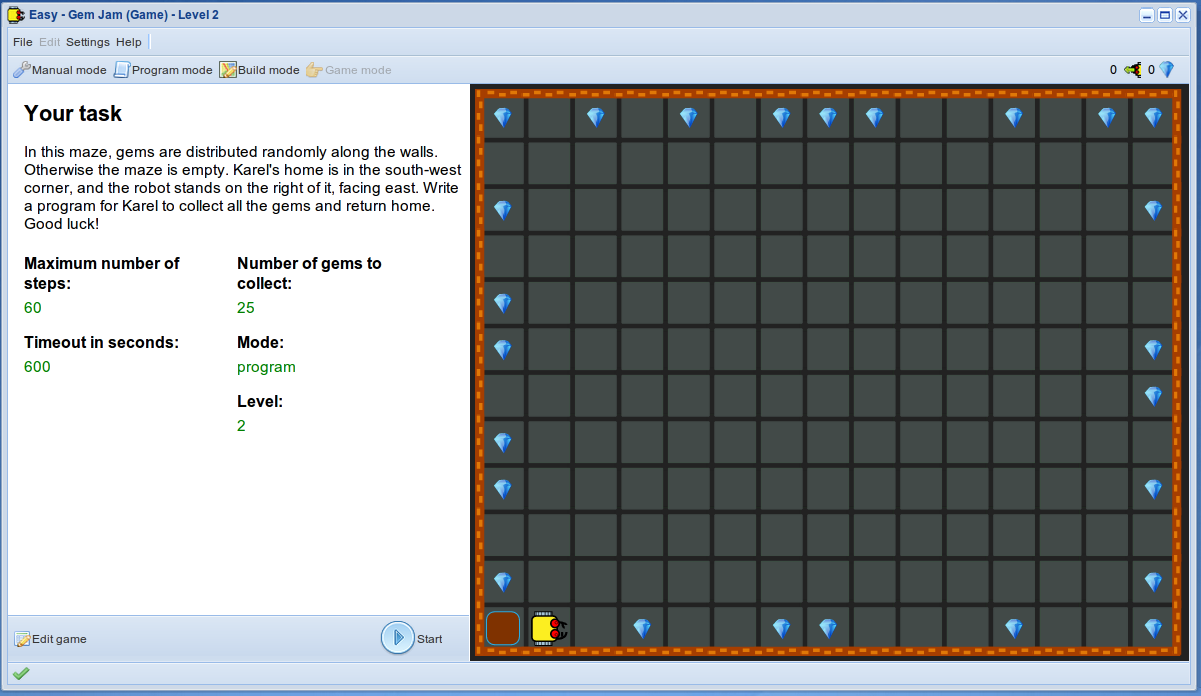
\includegraphics[width=0.7\textwidth]{img/game-gemjam.png}
\end{center}
\vspace{-4mm}
\caption{Gem Jam!}
\label{fig:gemjam}
\vspace{-10mm}
\end{figure}
\noindent

\subsection{Intermediate - Four Star Hotel}

{\em Before getting home, Karel has to collect all four stars of gems! }

\begin{figure}[!ht]
\begin{center}
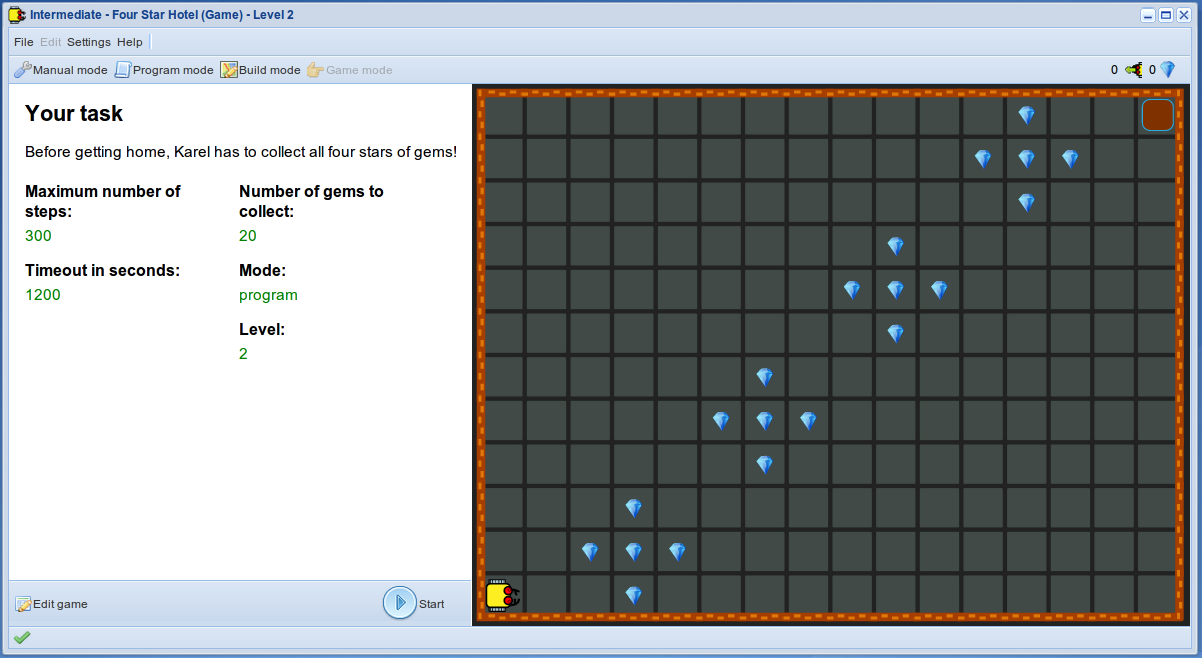
\includegraphics[width=0.7\textwidth]{img/game-fourstar.png}
\end{center}
\vspace{-4mm}
\caption{Four Star Hotel}
\label{fig:fourstar}
\vspace{-10mm}
\end{figure}
\noindent

\newpage

\subsection{Intermediate - The Matrix}

{\em Write a program for Karel to collect all gems and get back home! The record is 
210 steps made. Can you do it with fewer steps?}

\begin{figure}[!ht]
\begin{center}
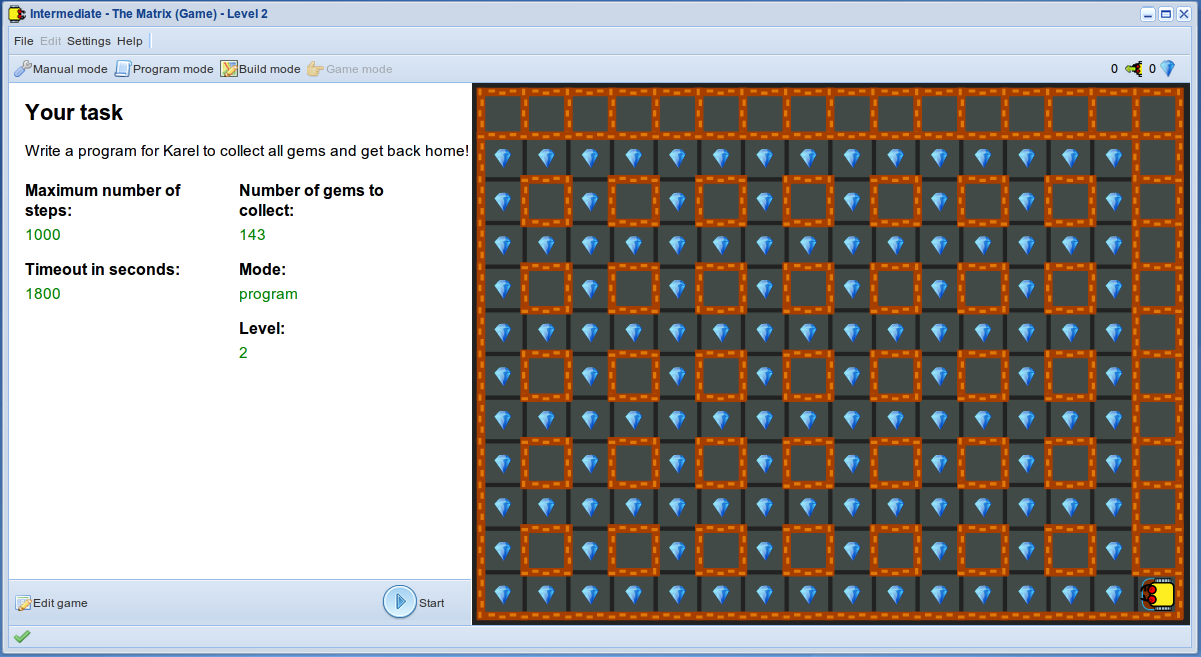
\includegraphics[width=0.7\textwidth]{img/game-matrix.png}
\end{center}
\vspace{-4mm}
\caption{The Matrix}
\label{fig:matrix}
\vspace{-10mm}
\end{figure}
\noindent

\subsection{Tough - Ariadne's Thread}

{\em In an ancient Greek legend, princess Ariadne saved the life of her 
beloved Theseus by giving him a thread that he used to avoid getting lost 
in the maze of king Minos and kill a feared beast Minotaurus. Karel uses 
a similar technique - he leaves behind him a chain of gems that helps him 
to safely find his way back home. }

\begin{figure}[!ht]
\begin{center}
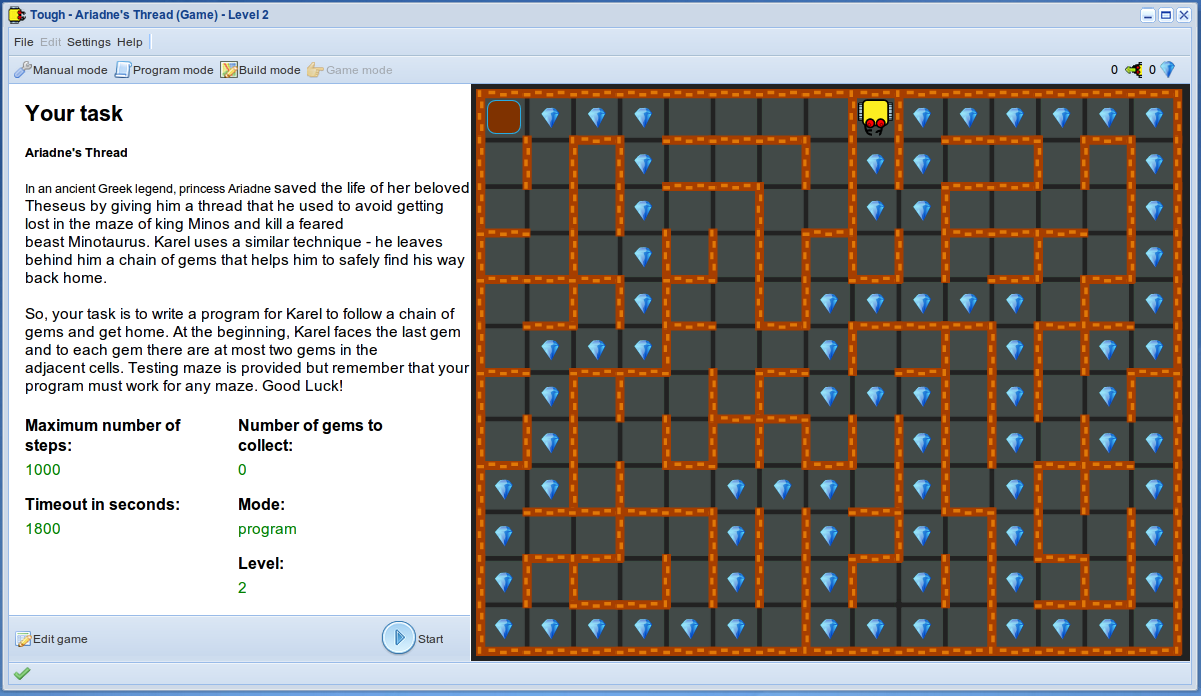
\includegraphics[width=0.7\textwidth]{img/game-ariadne.png}
\end{center}
\vspace{-4mm}
\caption{Maze of king Minos, home of the beast Minotaurus}
\label{fig:ariadne}
\vspace{-10mm}
\end{figure}
\noindent

\newpage

\subsection{Tough - Maze Patrol}

{\em Write a program for Karel to navigate through the maze using the 
right-hand rule. Do not forget to pick up all gems.}

\begin{figure}[!ht]
\begin{center}
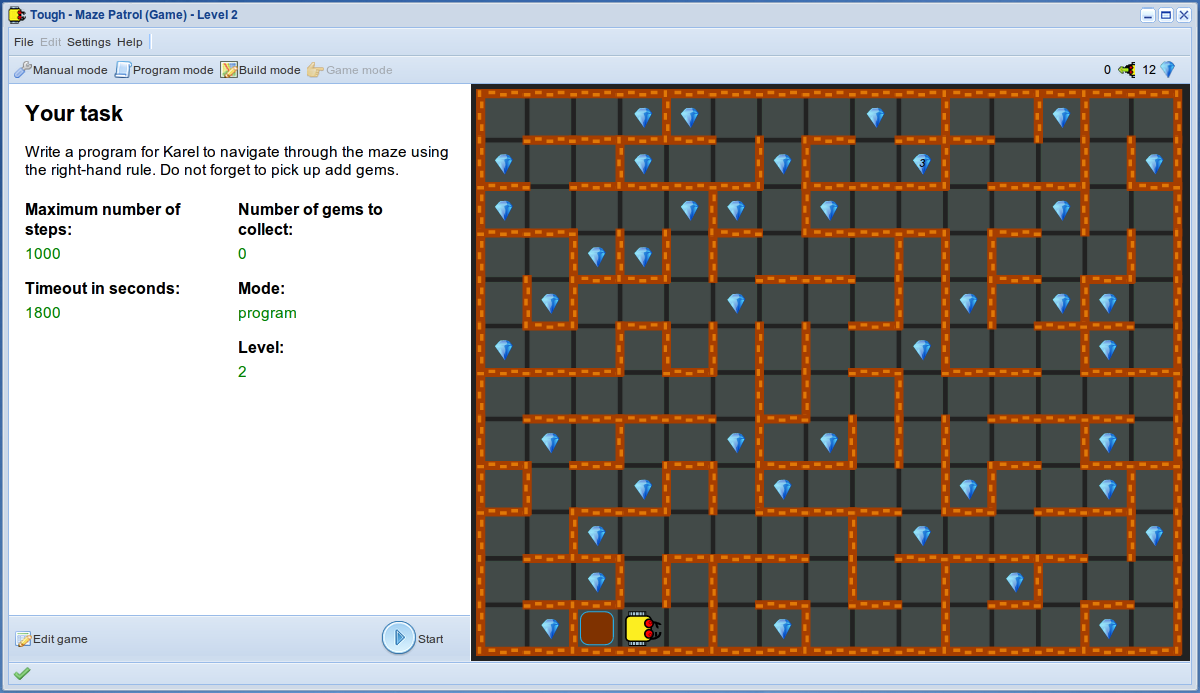
\includegraphics[width=0.7\textwidth]{img/game-patrol.png}
\end{center}
\vspace{-4mm}
\caption{Maze Patrol}
\label{fig:patrol}
\vspace{-10mm}
\end{figure}
\noindent

\newpage
\subsection{Very Tough - Eight Queens}

{\em Karel stands on an 8 x 8 chess board along with eight queens (the gems). Recall that a chess queen dominates its row, its column, as well as both diagonals that pass through her position. Nothing may stand in these fields or she will destroy it. Currently, some queens are threatening each other. Write a program for Karel to correct the positions of the queens in such a way that none of them is threatened. Your program should be able to do it for any initial distribution of the queens. Enter the home after you are finished.}

\begin{figure}[!ht]
\begin{center}
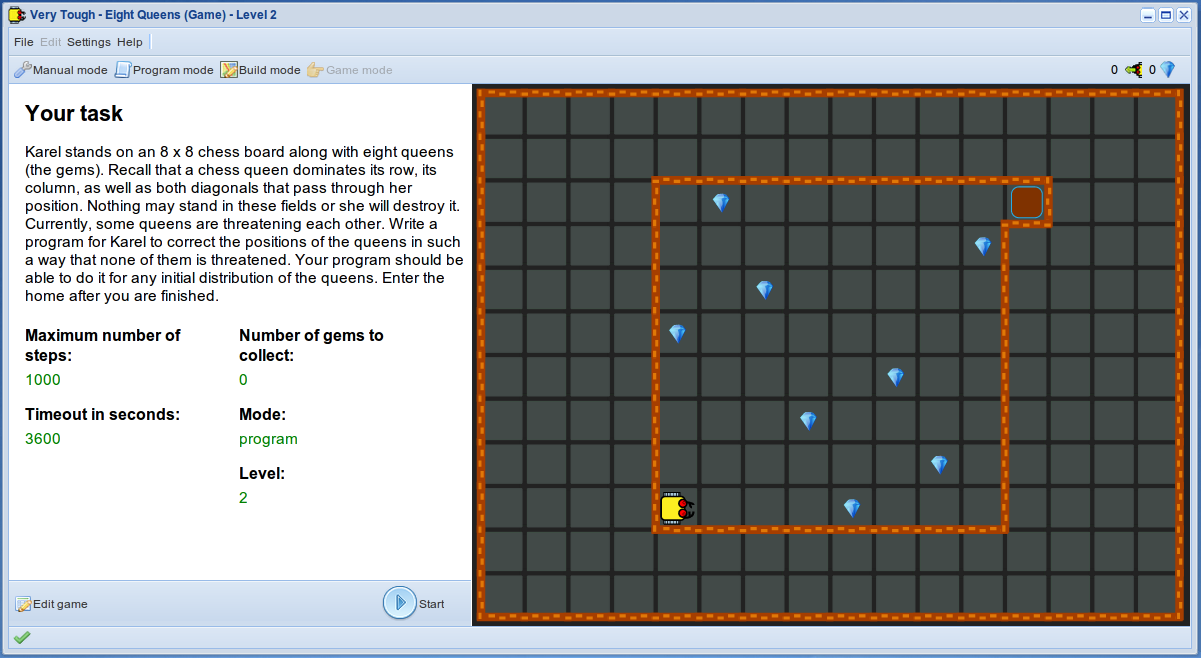
\includegraphics[width=0.7\textwidth]{img/game-queens.png}
\end{center}
\vspace{-4mm}
\caption{Eight Queens}
\label{fig:queens}
\vspace{-10mm}
\end{figure}
\noindent

\newpage
\subsection{Very Tough - Sorting Fun}

{\em Karel stands in front of six piles of gems. Each pile contains between one and 10 gems, and two or more piles can be equally large. The robot does not know how many gems are in each pile. Before getting home, the robot must sort them in such a way that the smallest pile is on the left and the largest on the right. }

\begin{figure}[!ht]
\begin{center}
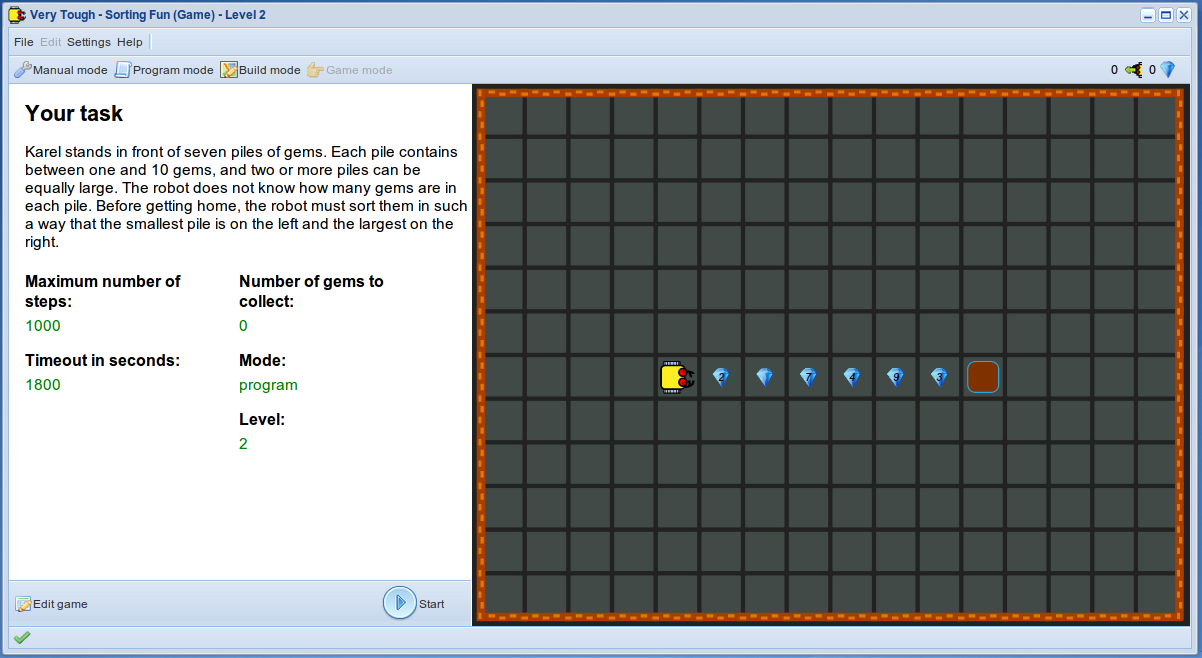
\includegraphics[width=0.7\textwidth]{img/game-sorting.png}
\end{center}
\vspace{-4mm}
\caption{Sorting Fun}
\label{fig:sorting}
\end{figure}
\noindent


\section{What To Do Next?}

Congratulations on making it to the end of the tutorial! We hope that you
enjoyed it. If you can think of any ways to improve the application 
Karel the Robot in NCLab or this tutorial, please let us know. If you 
feel capable of solving the last two problems, make sure to send us your 
solution. We are also thinking of creating a Gallery of Games just for Karel,
so if you have a nice game, please let us know as well. 

Although you may feel like an Almighty Programmer right now, we would
recommend staying humble. Even the most experienced programmers are
learning new things all the time. If you enjoy programming, your next 
language to learn may be Python. We have a Python Programming tutorial
in NCLab for you. We would also recommend that you learn Javascript since this 
is the most popular language for web development. Depending on your 
other hobbies or interests, C++ or even Fortran might be interesting. 
In any case, the NCLab Team wishes you good luck, and keep us in your 
favorite bookmarks!\\
\\
\hbox{} \hfill Your NCLab Team






\end{document}
